\documentclass[11pt,]{article}
\usepackage[left=1in,top=1in,right=1in,bottom=1in]{geometry}
\newcommand*{\authorfont}{\fontfamily{phv}\selectfont}
\usepackage[]{mathpazo}


  \usepackage[T1]{fontenc}
  \usepackage[utf8]{inputenc}



\usepackage{abstract}
\renewcommand{\abstractname}{}    % clear the title
\renewcommand{\absnamepos}{empty} % originally center

\renewenvironment{abstract}
 {{%
    \setlength{\leftmargin}{0mm}
    \setlength{\rightmargin}{\leftmargin}%
  }%
  \relax}
 {\endlist}

\makeatletter
\def\@maketitle{%
  \newpage
%  \null
%  \vskip 2em%
%  \begin{center}%
  \let \footnote \thanks
    {\fontsize{18}{20}\selectfont\raggedright  \setlength{\parindent}{0pt} \@title \par}%
}
%\fi
\makeatother




\setcounter{secnumdepth}{3}

\usepackage{longtable,booktabs}

\usepackage{graphicx,grffile}
\makeatletter
\def\maxwidth{\ifdim\Gin@nat@width>\linewidth\linewidth\else\Gin@nat@width\fi}
\def\maxheight{\ifdim\Gin@nat@height>\textheight\textheight\else\Gin@nat@height\fi}
\makeatother
% Scale images if necessary, so that they will not overflow the page
% margins by default, and it is still possible to overwrite the defaults
% using explicit options in \includegraphics[width, height, ...]{}
\setkeys{Gin}{width=\maxwidth,height=\maxheight,keepaspectratio}

\title{Estudio morfométrico fluvial de la cuenca Guayubín, República
Dominicana, en base a un modelo digital de elevación y algoritmos.  }



\author{\Large Darihana Linares Laureano\vspace{0.05in} \newline\normalsize\emph{Estudiante de Lic. en Geografía Mención Recursos Naturales y Ecoturismo,
en la Universidad Autónoma de Santo Domingo (UASD)}  }


\date{}

\usepackage{titlesec}

\titleformat*{\section}{\normalsize\bfseries}
\titleformat*{\subsection}{\normalsize\itshape}
\titleformat*{\subsubsection}{\normalsize\itshape}
\titleformat*{\paragraph}{\normalsize\itshape}
\titleformat*{\subparagraph}{\normalsize\itshape}

\titlespacing{\section}
{0pt}{36pt}{0pt}
\titlespacing{\subsection}
{0pt}{36pt}{0pt}
\titlespacing{\subsubsection}
{0pt}{36pt}{0pt}





\newtheorem{hypothesis}{Hypothesis}
\usepackage{setspace}

\makeatletter
\@ifpackageloaded{hyperref}{}{%
\ifxetex
  \PassOptionsToPackage{hyphens}{url}\usepackage[setpagesize=false, % page size defined by xetex
              unicode=false, % unicode breaks when used with xetex
              xetex]{hyperref}
\else
  \PassOptionsToPackage{hyphens}{url}\usepackage[unicode=true]{hyperref}
\fi
}

\@ifpackageloaded{color}{
    \PassOptionsToPackage{usenames,dvipsnames}{color}
}{%
    \usepackage[usenames,dvipsnames]{color}
}
\makeatother
\hypersetup{breaklinks=true,
            bookmarks=true,
            pdfauthor={Darihana Linares Laureano (Estudiante de Lic. en Geografía Mención Recursos Naturales y Ecoturismo,
en la Universidad Autónoma de Santo Domingo (UASD))},
             pdfkeywords = {Geomorfología fluvial, Morfometria de cuencas, Análisis hortoniano,
Índice de concavidad, Perfil longitudinal, Patrones de drenaje},  
            pdftitle={Estudio morfométrico fluvial de la cuenca Guayubín, República
Dominicana, en base a un modelo digital de elevación y algoritmos.},
            colorlinks=true,
            citecolor=blue,
            urlcolor=blue,
            linkcolor=magenta,
            pdfborder={0 0 0}}
\urlstyle{same}  % don't use monospace font for urls

% set default figure placement to htbp
\makeatletter
\def\fps@figure{htbp}
\makeatother

\usepackage{pdflscape} \newcommand{\blandscape}{\begin{landscape}}
\newcommand{\elandscape}{\end{landscape}}


% add tightlist ----------
\providecommand{\tightlist}{%
\setlength{\itemsep}{0pt}\setlength{\parskip}{0pt}}

\begin{document}
	
% \pagenumbering{arabic}% resets `page` counter to 1 
%
% \maketitle

{% \usefont{T1}{pnc}{m}{n}
\setlength{\parindent}{0pt}
\thispagestyle{plain}
{\fontsize{18}{20}\selectfont\raggedright 
\maketitle  % title \par  

}

{
   \vskip 13.5pt\relax \normalsize\fontsize{11}{12} 
\textbf{\authorfont Darihana Linares Laureano} \hskip 15pt \emph{\small Estudiante de Lic. en Geografía Mención Recursos Naturales y Ecoturismo,
en la Universidad Autónoma de Santo Domingo (UASD)}   

}

}








\begin{abstract}

    \hbox{\vrule height .2pt width 39.14pc}

    \vskip 8.5pt % \small 

\noindent El estudio morfométrico de cuencas fluviales son sumamente importantes
para comprender la configuracion de la misma. A pesar de esto los
estudios de esta categoria realizados en el pais son muy escasos, aun
teniendo una hidrografía rica, esperando a ser explorada y analizada. El
estudio morfométrico de la cuenca Guayubín (773.56 km
extsuperscript\{2\}), señala la existencia de una relacion entre la red
de drenaje con la litologia el el area de cuenca, que explica la forma
peculiar d la primera. De la misma manera como a traves de indices es
posible explicar los fenómenos descubiertos que se producen en la
cuenca, en el caso de captura fluvial. Esta investigación evidencia la
eficacia de la tecnologia geoespacial para el estudio cuantitavo de una
cuenca hidrografica, independientemente del tamaño de la misma, asi
como, que esta tecnica es posibe aplicarla en el pais a bajo costo y
produciendo informacion de alta calidad.


\vskip 8.5pt \noindent \emph{Keywords}: Geomorfología fluvial, Morfometria de cuencas, Análisis hortoniano,
Índice de concavidad, Perfil longitudinal, Patrones de drenaje \par

    \hbox{\vrule height .2pt width 39.14pc}



\end{abstract}


\vskip 6.5pt


\noindent  \section{Introducción}\label{introducciuxf3n}

Desde hace siglos atrás el hombre ha buscado la manera de explicar y
entender las distintas formas que el paisaje terrestre (relieve) posee.
Autores numerosos han investigado la génesis de estas nociones
geomorfológicas, remontándose a tres siglos atrás. Autores como Hutton,
Playfair y Lyell, sirvieron de antecesores o bases para la ciencia
geomorfológica. Tras su consolidación como ciencia en Francia numerosos
autores fueron demostrando la importancia de esta ciencia, incluso
ramificándola (climática, eólica, litoral, glaciar, estructural,
tectónica, kárstica y fluvial; siendo la última de interés para esta
investigación), para mayor eficacia en sus estudios.

Los estudios en la geomorfología fluvial a nivel mundial son numerosos y
han servido para explicar cómo los drenajes de los ríos y sus redes
hidrográficas son importantes para la geomorfología, ya que estas redes
fluviales son parte de los procesos de modelado más activos en la
formación del relieve y que permiten mensurar la configuración del
mismo. Para los estudios en geomorfología fluvial, se hace uso del
análisis morfométrico de cuencas hidrográficas. La morfometría de cuenca
se ha convertido en la técnica cuantitativa para el estudio de las
cuencas de manera detallada y ordenada. Actualmente en la República
Dominicana el uso del análisis morfométrico para estudiar cuencas
hidrográficas es poco e insuficiente, a pesar de que la República
Dominicana goza de una diversa y extensa red de cuencas hidrográficas,
ricas y aprovechables para la aplicación de diversas técnicas con el fin
de explicar y entender las propiedades del relieve y su relación con las
cuencas fluviales. Por lo que, este estudio es un aporte para dar a
conocer la configuración y modelado de la cuenca hidrográfica del rio
Guayubín, con el fin de fijar parámetros que permitan evaluar esta
cuenca fluvial; identificando el aspecto general de la cuenca y de la
red, el orden de red y análisis hortoniano, los perfiles longitudinales
e índice de concavidad de cursos más largos, y la morfometría de cuenca.
En ese mismo orden es imprescindible conocer el concepto de cuenca
fluvial o de drenaje, que no es más que el conjunto de cuerpos de agua
con un área determinada que fluyen por distintos canales y escurren en
un mismo desagüe. Según los autores Gregory y Walling, 1973; y Chorley,
1969 (como citó Gutiérrez Elorza (2008)), una cuenca fluvial compone el
espacio determinado en el que se suministran las aguas que discurren por
la superficie, el mismo está delimitado tanto por su relieve y su
hidrología. También considerada como una unidad imprescindible en
geomorfológica.

\subsection{Revisión bibliográfica}\label{revisiuxf3n-bibliogruxe1fica}

El aspecto general de la cuenca y de la red se refiere a los parámetros
hidrográficos que posee la cuenca (la acumulación de flujos y cálculo de
su umbral, elevación, depresión, y otros). Según Castillo (2015), la
acumulación de flujos señala a todas las celdas que desaguan en una en
particular, la misma se adquiere partiendo de la dirección de la
corriente o flujo. Venkatachalam et al. (2001) dicen que la acumulación
de flujo de una celda se instituye de acuerdo con la sumatoria de los
valores de la acumulación de flujo de las celdas próximas que drenan en
ella. En cuanto al umbral, según ESRI (2012), se es necesario un ráster
de acumulación de flujo y la `porción mínima de celdas que componen una
corriente de agua. También se refiere a la forma que adquiere la cuenca
y a la forma de su red de drenaje, según la conformación de sus ríos y
el material rocoso que la compone (patrones de drenaje). Varios autores
expresan que existe una conexión entre la estructura que posee la red de
drenaje con el material rocoso (Pedraza Gilsanz (1996), Gutiérrez Elorza
(2008), Howard (1967), Gregory \& Walling (1973)).

El orden de red hace referencia al orden en el que se clasifican los
cursos de agua, todo en base a su ramificación. Según Wikipedia (2020),
el orden de un curso de agua es siempre un número entero positivo que se
usa tanto en Geomorfología como en Hidrología para denotar la magnitud
de ramificación que posee una red fluvial. Para Bowden \& Wallis (1964),
el orden de red sostiene una relación entre las rocas con la
configuración de la red fluvial y con los procesos tanto hidrológicos
como erosivos. La clasificación de la red se hace de manera jerárquica.
Hoy día existen múltiples normas para determinar la jerarquía de una
red: Strahler (1952), Horton (1945), Shreve (1967), Scheidegger (1970),
Leopold et al. (1964) Hack (1957) y Topological.

Dice Pinilla (1993) que para los años 40 el análisis hortoniano había
sentado las bases de lo que hoy es la morfometría fluvial; por lo que la
aplicación del análisis hortoniano al estudio de cuencas hidrográficas
son imprescindibles. Para Horton (1945), la razón de bifurcación resulta
ser la conexión entre el número de redes fluviales de una jerarquía
asignada entre el número de redes de jerarquía mayor próxima, y se;ala
que esta casi siempre es constante para los ordenes de red de una
cuenca.

El perfil longitudinal de un curso de agua es una línea adquirida al
representar las diversas alturas que se presentan desde el nacimiento de
este hasta donde desagua (Gutiérrez Elorza (2008)). Según Pedraza
Gilsanz (1996), por medio de los perfiles longitudinales es posible
fundamentar definiciones en segmentos con geometría heterogénea
(cóncavo, convexo y rectilíneo), o pendiente; las acomodaciones para
cada parte a una función matemática; e incluso análisis geométricos
basados en elementos físicos o evolutivos. Gutiérrez Elorza (2008), dice
que el perfil longitudinal es generalmente cóncavo, aunque esta
concavidad no está clara para muchos cursos fluviales. En cuanto al
índice de concavidad, este no es más que un indicador que hace posible
la evaluación del nivel de torcedura o curvatura del perfil longitudinal
(Garzón Heydt, Ortega, Garrote, \& others (n.d.)). Se calcula así, la
superficie debajo del perfil longitudinal es extraída del total del área
debajo del segmento que conecta los dos límites del perfil (Goldrick \&
Bishop (2007)).

El análisis morfométrico abarca un conjunto de índices morfológicos que
apuntan a un análisis detallado y cuantitativo de cuencas hidrográficas
(Morais \& Almeida (2010)). El análisis morfométrico de cuencas
hidrográficas se inicia por la ordenación de canales fluviales, con la
finalidad de establecer una jerarquía fluvial. Esta, a su vez, consiste
en el proceso de establecer la clasificación de determinado curso de
agua (o el área drenada que le pertenece) en el conjunto total de la
cuenca hidrográfica en la que se encuentra. Aunque, según el autor, esto
se logra con la función de facilitar y volver más objetivos los estudios
morfométricos sobre las cuencas hidrográficas (Christofoletti (1988)).
En cuanto a la curva hipsométrica de una cuenca Strahler (1952) dice que
el porcentaje de la curva hipsométrica no es más que la relación entre
el área de la sección diagonal horizontal de una red de drenaje con una
altitud relativa sobre la boca de la cuenca, e incluso estas curvas
pueden ser explicadas y relacionadas a través del uso de parámetros
bidimensionales. Y referente a la integral Hipsométrica, Fernandez \&
Rocha (2016) expresa que el cálculo de este índice mide como está
distribuida la altitud en una cuenca fluvial.

Este estudio proporciona nueva información sobre la cuenca del río
Guayubín en el campo de Morfometría fluvial, sabiendo que este es el
primer estudio morfométrico que se le realiza a la cuenca; y además este
posee un script el cual permite su reproducción sin coste alguno.

Preguntas de Investigación:

¿Qué forma posee la cuenca y su red de drenaje?

¿Cómo se organiza la red de drenaje?

¿Existe algun pratrón en la forma de de cuenca y red de drenaje por
ordenes?

¿Se produce el fenómeno de constancia en la razón de bifurcación?

¿Se produce la relación de perfiles longitudinales e índice de
concavidad con la litología en la cuenca?

¿Hay una relación entre los parámetros morfométricos con las
características litológica y estructural de cuenca?

¿Con qué factores se asocian la curva e integral hipsométricas de la
cuenca?

\section{Área de estudio}\label{uxe1rea-de-estudio}

La cuenca del río Guayubín se encuentra entre las morforegiones
Cordillera Central y Valle del Cibao Occidental, en la República
Dominicana (latitud 19.46\(^\circ\)N, longitud -71.41\(^\circ\)W), entre
las provincias Santiago Rodríguez, Monte Cristi y Dajabón. En la
provincia Dajabón engloba de forma completa el municipio El Pino, y de
manera parcial los municipios Loma de Cabrera y Partido; en la provincia
Monte Cristi contiene parcialmente los municipios Las Matas de Santa
Cruz y Guayubín; y en la provincia Santiago Rodríguez comprende los
municipios Villa Los Almácigos y San Ignacio de Sabaneta. Los municipios
más poblados en el interior de la cuenca son Guayubín (35,923 hab.), San
Ignacio de Sabaneta (34,540 hab), y Loma de Cabrera (15,624 hab). (Ver
figura \ref {mapacuenca}).

La cuenca del río Guayubín, según Medio Ambiente y Recurso Naturales
(2015), abarca una área de 770.35 km\textsuperscript{2}. De acuerdo con
el mapa de Medio Ambiente y Recurso Naturales (2015), la cabecera del
rio Guayubín se ubica en la vertiente noroeste de el Cerro La Pelada, en
un paraje denominado Palo Amarillo; mientras que sus aguas se vierten en
el río Yaque del Norte, en la localidad Guayubín.

\begin{figure}
\centering
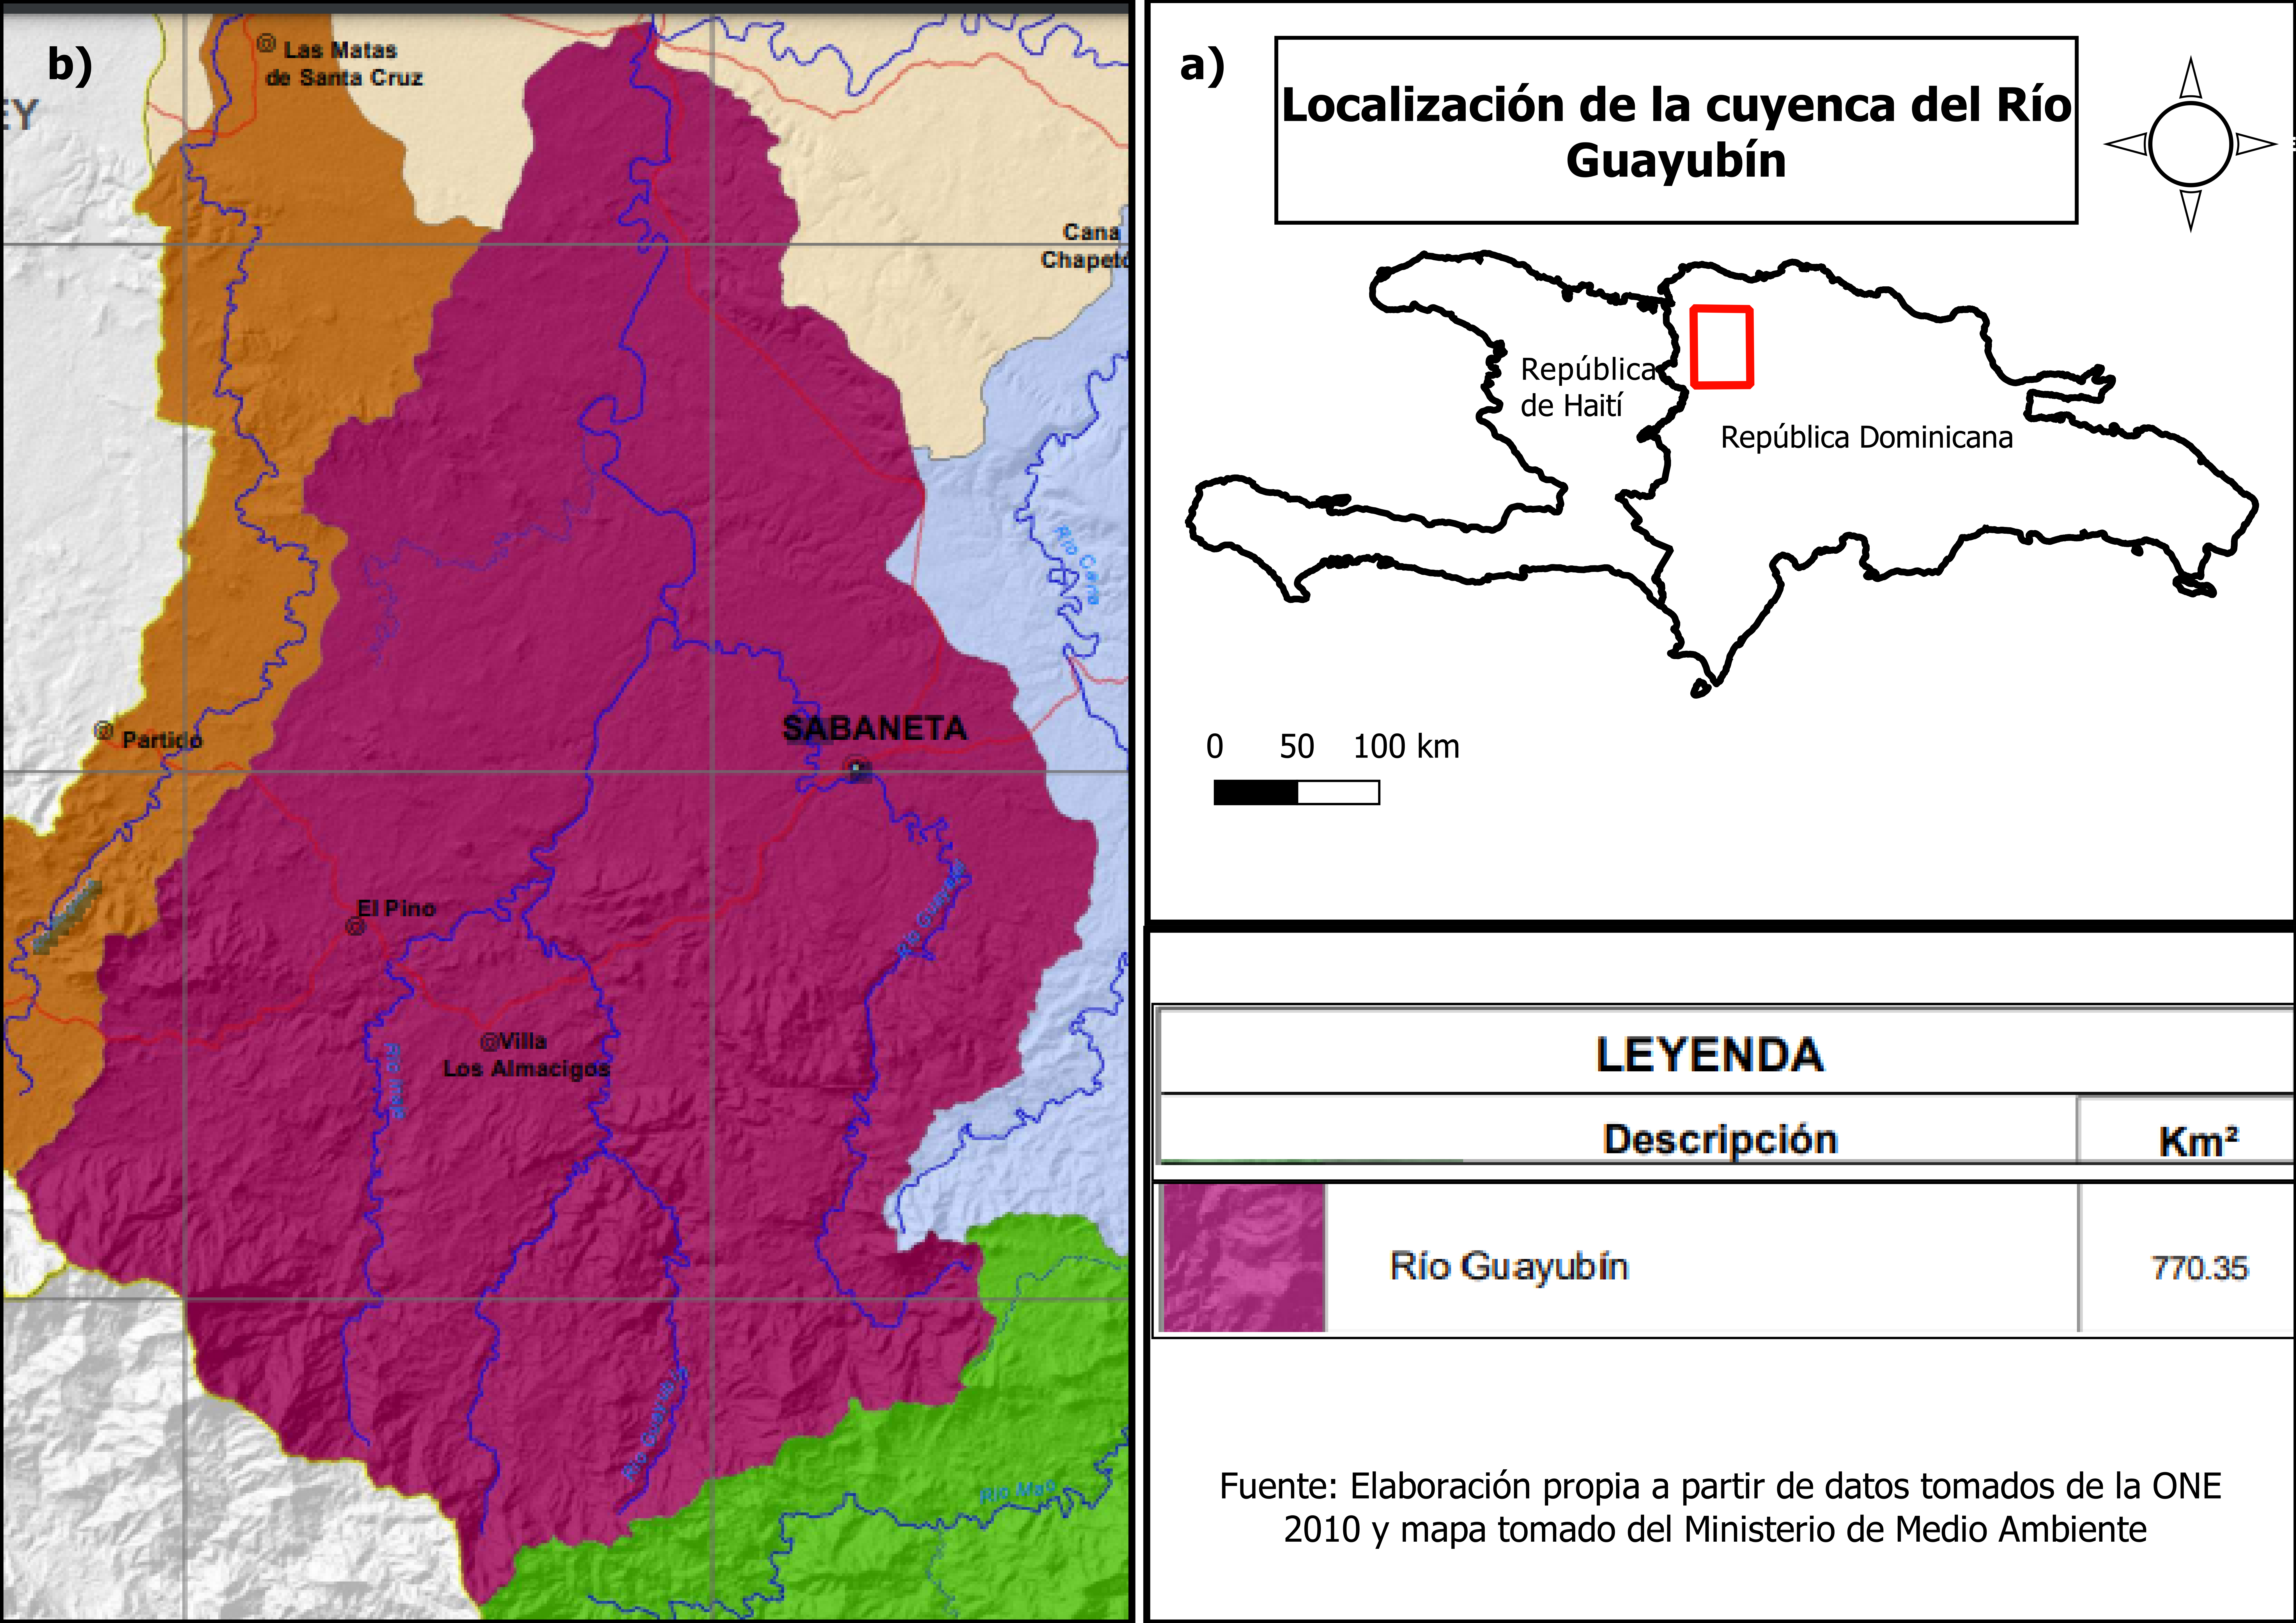
\includegraphics[width=1.00000\textwidth]{Mapa final.png}
\caption{Cuenca del río Guayubín\label{mapacuenca}}
\end{figure}

\begin{figure}
\centering
\includegraphics[width=0.60000\textwidth]{geologico.png}
\caption{Mapa Geologico de la cuenca\label{magecu}}
\end{figure}

\section{Materiales y Metodología}\label{materiales-y-metodologuxeda}

Para el estudio morfométrico de la cuenca Guayubín se usó softwares de
código abierto como medio para procesar datos estadísticos y modelos
digitales con la finalidad de generar las informaciones a analizar e
interpretar. Ver materiales en tabla\ref{tab:materiales}.

\begin{longtable}[]{@{}cc@{}}
\caption{\label{tab:materiales} Materiales utilizados en la
investigacion.}\tabularnewline
\toprule
\begin{minipage}[b]{0.11\columnwidth}\centering\strut
Materiales\strut
\end{minipage} & \begin{minipage}[b]{0.83\columnwidth}\centering\strut
Uso\strut
\end{minipage}\tabularnewline
\midrule
\endfirsthead
\toprule
\begin{minipage}[b]{0.11\columnwidth}\centering\strut
Materiales\strut
\end{minipage} & \begin{minipage}[b]{0.83\columnwidth}\centering\strut
Uso\strut
\end{minipage}\tabularnewline
\midrule
\endhead
\begin{minipage}[t]{0.11\columnwidth}\centering\strut
RStudio\strut
\end{minipage} & \begin{minipage}[t]{0.83\columnwidth}\centering\strut
se redactó el manuscrito, se procesaron los datos que extraídos del DEM
de la cuenca a través de un script.\strut
\end{minipage}\tabularnewline
\begin{minipage}[t]{0.11\columnwidth}\centering\strut
library rgrass7\strut
\end{minipage} & \begin{minipage}[t]{0.83\columnwidth}\centering\strut
se creó una interfaz que permitió establecer una conexión entre la
version 7 del sistema de infromacion geográfica GRASS, y R, que crea un
entorno GRASS desechable dentro de R.\strut
\end{minipage}\tabularnewline
\begin{minipage}[t]{0.11\columnwidth}\centering\strut
library sp\strut
\end{minipage} & \begin{minipage}[t]{0.83\columnwidth}\centering\strut
este paquete se utilizó para la importación, manipulación y exportación
de datos espaciales en R, y para imprimir / mostrar de los mismos.\strut
\end{minipage}\tabularnewline
\begin{minipage}[t]{0.11\columnwidth}\centering\strut
library sf\strut
\end{minipage} & \begin{minipage}[t]{0.83\columnwidth}\centering\strut
con esto se crearon caracteristicas simples (simple features), que
amplían los objetos tipo data.frame con una columna de lista de
características simples.\strut
\end{minipage}\tabularnewline
\begin{minipage}[t]{0.11\columnwidth}\centering\strut
library raster\strut
\end{minipage} & \begin{minipage}[t]{0.83\columnwidth}\centering\strut
este paquete se usó para manipular datos geográficos (espaciales) en
formato `ráster'.\strut
\end{minipage}\tabularnewline
\begin{minipage}[t]{0.11\columnwidth}\centering\strut
library leaflet\strut
\end{minipage} & \begin{minipage}[t]{0.83\columnwidth}\centering\strut
esta función se utilizó para representar los vectores y rásters\strut
\end{minipage}\tabularnewline
\begin{minipage}[t]{0.11\columnwidth}\centering\strut
library leafem\strut
\end{minipage} & \begin{minipage}[t]{0.83\columnwidth}\centering\strut
se usó para proveer una extensión para leaflet usados para paquetes
mapview, permite mostrar las coordenadas de la posición del puntero del
mouse, consultar valores de imagen a través de puntero del mouse y
botones de zoom a capa.\strut
\end{minipage}\tabularnewline
\begin{minipage}[t]{0.11\columnwidth}\centering\strut
library mapview\strut
\end{minipage} & \begin{minipage}[t]{0.83\columnwidth}\centering\strut
el paquete permitió ver los objetos espaciales de forma
interactiva.\strut
\end{minipage}\tabularnewline
\begin{minipage}[t]{0.11\columnwidth}\centering\strut
library readr\strut
\end{minipage} & \begin{minipage}[t]{0.83\columnwidth}\centering\strut
se utilizó pata leer datos rectangulares (como `csv', `tsv' y
`fwf').\strut
\end{minipage}\tabularnewline
\begin{minipage}[t]{0.11\columnwidth}\centering\strut
QGIS with GRASS\strut
\end{minipage} & \begin{minipage}[t]{0.83\columnwidth}\centering\strut
se usó para la visualización de vectores y rasters generados con RStudio
en una región de GRASS, y la visualización de los mapas Topológicos y
Geológicos de la República Dominicana, tambien, para la creación de
algunos mapas de localización.\strut
\end{minipage}\tabularnewline
\begin{minipage}[t]{0.11\columnwidth}\centering\strut
Google Earth\strut
\end{minipage} & \begin{minipage}[t]{0.83\columnwidth}\centering\strut
para observar datos en formato kml generados y exportados de RStudio y
asi como la representacion del relieve del lugar de estudio.\strut
\end{minipage}\tabularnewline
\begin{minipage}[t]{0.11\columnwidth}\centering\strut
Mapa Topológico de RD\strut
\end{minipage} & \begin{minipage}[t]{0.83\columnwidth}\centering\strut
se utilizó para hacer comparaciones y obtener referencias sobre el
relieve.\strut
\end{minipage}\tabularnewline
\begin{minipage}[t]{0.11\columnwidth}\centering\strut
Mapa Geológico Nacional de RD\strut
\end{minipage} & \begin{minipage}[t]{0.83\columnwidth}\centering\strut
se usó para hacer comparaciones y obtener referencias sobre la
composición rocosa y los años que datan estas (ver
figura\ref{magecu}).\strut
\end{minipage}\tabularnewline
\bottomrule
\end{longtable}

\subsection{Metodología}\label{metodologuxeda}

Para el desarrollo del estudio lo primero a realizar fue crear una
región de GRASS en R, importar fuentes y definir la extensión y
resolución (DEM). Luego, explorar básicos entre GRASS y R.

\subsubsection{Aspecto de la cuenca y de la red de
drenaje.}\label{aspecto-de-la-cuenca-y-de-la-red-de-drenaje.}

Los parámetros de la cuenca fueron calculados por medio del addon de
GRASS GIS \texttt{r.watershed} (Charles Ehlschlaeger (2003--2021b)),
utilizando un Dem. Los parámetros calculados fueron acumulación,
elevación, depresión, drenaje, flujo, cuenca y media cuenca, con un
umbral de acumulación de flujo de 80 celdas necesarias para que exista
una red de agua. Luego, las capas generadas fueron ingresadas a R con la
\texttt{librería\ sp} y manejadas con la \texttt{librería\ raster}. Se
usó el addon \texttt{r.water.outlet} (Charles Ehlschlaeger
(2003--2021a)) para la extracción de la cuenca se usaron los parámetros
siguientes: de entrada un mapa de dirección de drenajes (creado con el
addon \texttt{r.watershed}), de coordenadas de desembocadura de la
cuenca (obtenidas con la \texttt{librería\ Mapview}), y de salida el
nombre de la cuenca. Así mismo, se usó el addon \texttt{r.to.vect} (Team
(2003--2021)), para convertir el ráster resultante en vectorial, con los
parámetros a continuación: de entrada el mapa ráster de la cuenca, de
salida el nombre del vectorial y para la característica de salida se usó
el área. Al final de la operación los resultados fueron llevados a R.
Para extraer la red de drenaje se aplicó el addon
\texttt{r.stream.extract} (Metz (2003--2021)), usando los parámetros:
elevación, umbral de acumulación, mapa ráster de flujos y mapa vectorial
de flujos. Luego los resultados de este procedimiento fueron llevados a
R.

\subsubsection{Orden de red y análisis
hortoniano.}\label{orden-de-red-y-anuxe1lisis-hortoniano.}

En cuanto al orden de red y el análisis hortoniano, se usó el addon
\texttt{r.stream.extract} (Metz (2003--2021)), para producir un mapa de
dirección de flujo con los parámetros: de entrada un modelo de
elevación, un umbral de acumulación y de salida el nombre del mapa. Para
la creación de mapas de ordenes de redes generados con
\texttt{r.stream.order} (Jasiewicz (2003--2021)) se usaron los
parámetros: de entrada un mapa ráster de red de arroyos, un modelo de
elevación, un mapa de dirección de flujos, un mapa de acumulación, de
salida un vector con todos los atributos de los flujos, y a salida de
los vectores con los órdenes de redes según Strahler, Horton, Shreve,
Hack y Topo. Para analizar el orden de red de la cuenca se utilizó la
clasificación de Strahler. Mientras que se usaron los addons
\texttt{r.info} (Michael O'Shea (2003--2021)), para obtener los valores
mínimos y máximos del orden de red según Strahler a partir de un ráster;
para delimitar la cuenca a través de la red de drenaje se utilizó
\texttt{r.stream.basins} (Jarek Jasiewicz \& Institute (2003--2021a)),
los parámetros usados son: de entrada un mapa de dirección de flujos, un
mapa mascara de flujos, rango de valores de categorías, y de salida el
nombre del mapa. En cuanto a las estadísticas según orden de red de
Horton para las redes de Strahler y Horton se usó el addon
\texttt{r.stream.stats} (Jarek Jasiewicz \& Institute (2003--2021b)),
para resumir las estadísticas; los parámetros a usados fueron: de
entrada un ráster de red de arroyos, un ráster de dirección de flujos,
un modelo de elevación y de salida el nombre del archivo.

\subsubsection{Índices de concavidad y perfiles
longitudinales.}\label{uxedndices-de-concavidad-y-perfiles-longitudinales.}

Para calcular los índices de concavidad y los perfiles longitudinales,
primero, se obtuvieron los cursos más largos de la cuenca a través de la
función \texttt{LfpNetwork} (José Ramón Martínez Batlle (2018b)), usando
coordenadas de desembocadura de la cuenca obtenidas con la
\texttt{librería\ Mapview}, vectores de ordenes de red, mapa de flujo de
dirección y un sufijo de salida para los resultados que se generen.
Segundo, para producir los perfiles longitudinales e índices de
concavidad se empleó la función \texttt{LfpProfilesConcavity} (José
Ramón Martínez Batlle (2018c)), utilizando como parámetro la red de
cursos de agua más largos, coordenadas de desembocadura, un dem, un mapa
de flujos de drenaje, un prefijo, un sistema de referencia de
coordenadas, un parámetro de suavizado y un número de filas de los
perfiles.

\subsubsection{Morfometría de cuenca.}\label{morfometruxeda-de-cuenca.}

Tras crear una nueva región de GRASS en R, se continuó con convertir a
números enteros la extensión y la resolución del DEM con las funciones
\texttt{integerextent} (José Ramón Martínez Batlle (2020a)), y
\texttt{xyvector} (José Ramón Martínez Batlle (2018d)). También, se usó
la herramienta \texttt{gdalwarp} (Frank Warmerdam \& others
(1998--2021)), para reproyectar y deformar ráster. Se utilizaron los
addons \texttt{g.proj} (Kelly (2003--2021)), y \texttt{r.in.gdal}
(Warmerdam (2003--2021)), para importar a la sesión de GRASS. Se usó el
addon \texttt{r.stream.extract} (Metz (2003--2021)), para generar una
red de drenaje y obtener coordenadas a continuación, y que serían,
luego, transformadas a EPSG (MappingGis (2016)), como número entero con
la función \texttt{My\_Trans} (José Ramón Martínez Batlle (2020b)). En
cuanto a la obtención de los parámetros morfométricos de la cuenca se
usa el addon \texttt{r.basin} (Margherita Di Leo (2003--2021)), con los
parámetros siguientes: un modelo de elevación, un prefijo de salida,
coordenadas de la salida de la cuenca, umbral de acumulación, y un
directorio donde se ubicará el archivo de salida. Los vectores obtenidos
son transformados a EPGS (MappingGis (2016)), y asi visualizar con la
\texttt{librería\ Leaflet}. Y para poder explorar los parámetros de la
cuenca se usó la \texttt{librería\ Readr}. Finalmente, para el cálculo
de la curva y la integral hipsométrica, lo primero fue representar las
cuencas con las librerías \texttt{Sp} y \texttt{Mapview}; y segundo,
calcular la integral y curva hipsométrica utilizando la función
\texttt{HypsoIntCurve} (José Ramón Martínez Batlle (2018a)), usando de
parámetros los vectores de arroyos de cuenca de orden 2 y 3, un modelo
de elevación, un asignador de campos, el número de filas y una etiqueta
de tamaño.

\section{Resultados}\label{resultados}

El fruto del estudio realizado a la cuenca del río Guayubín aplicando la
metodología anterior, produce información que facilita el análisis y
comprensión de la cuenca fluvial, tanto de manera agrupada, como de
forma desagregada.

\subsection{Aspecto general de la cuenca y de la red de
drenaje.}\label{aspecto-general-de-la-cuenca-y-de-la-red-de-drenaje.}

Los resultados arrojados por el estudio muestran que la cuenca del río
Guayubín tiene una área de 773.56 km\textsuperscript{2}, y un perímetro
de 156.12 km (Ver tablas \ref{tab:estadisticaor} y
\ref{tab:parametrosm}). La cuenca tiene forma de pera y su red drenaje
presenta patrones denditricos (ver figura\ref{cuencavectorial} y
figura\ref{red de drenaje extraida}).

\begin{figure}
\centering
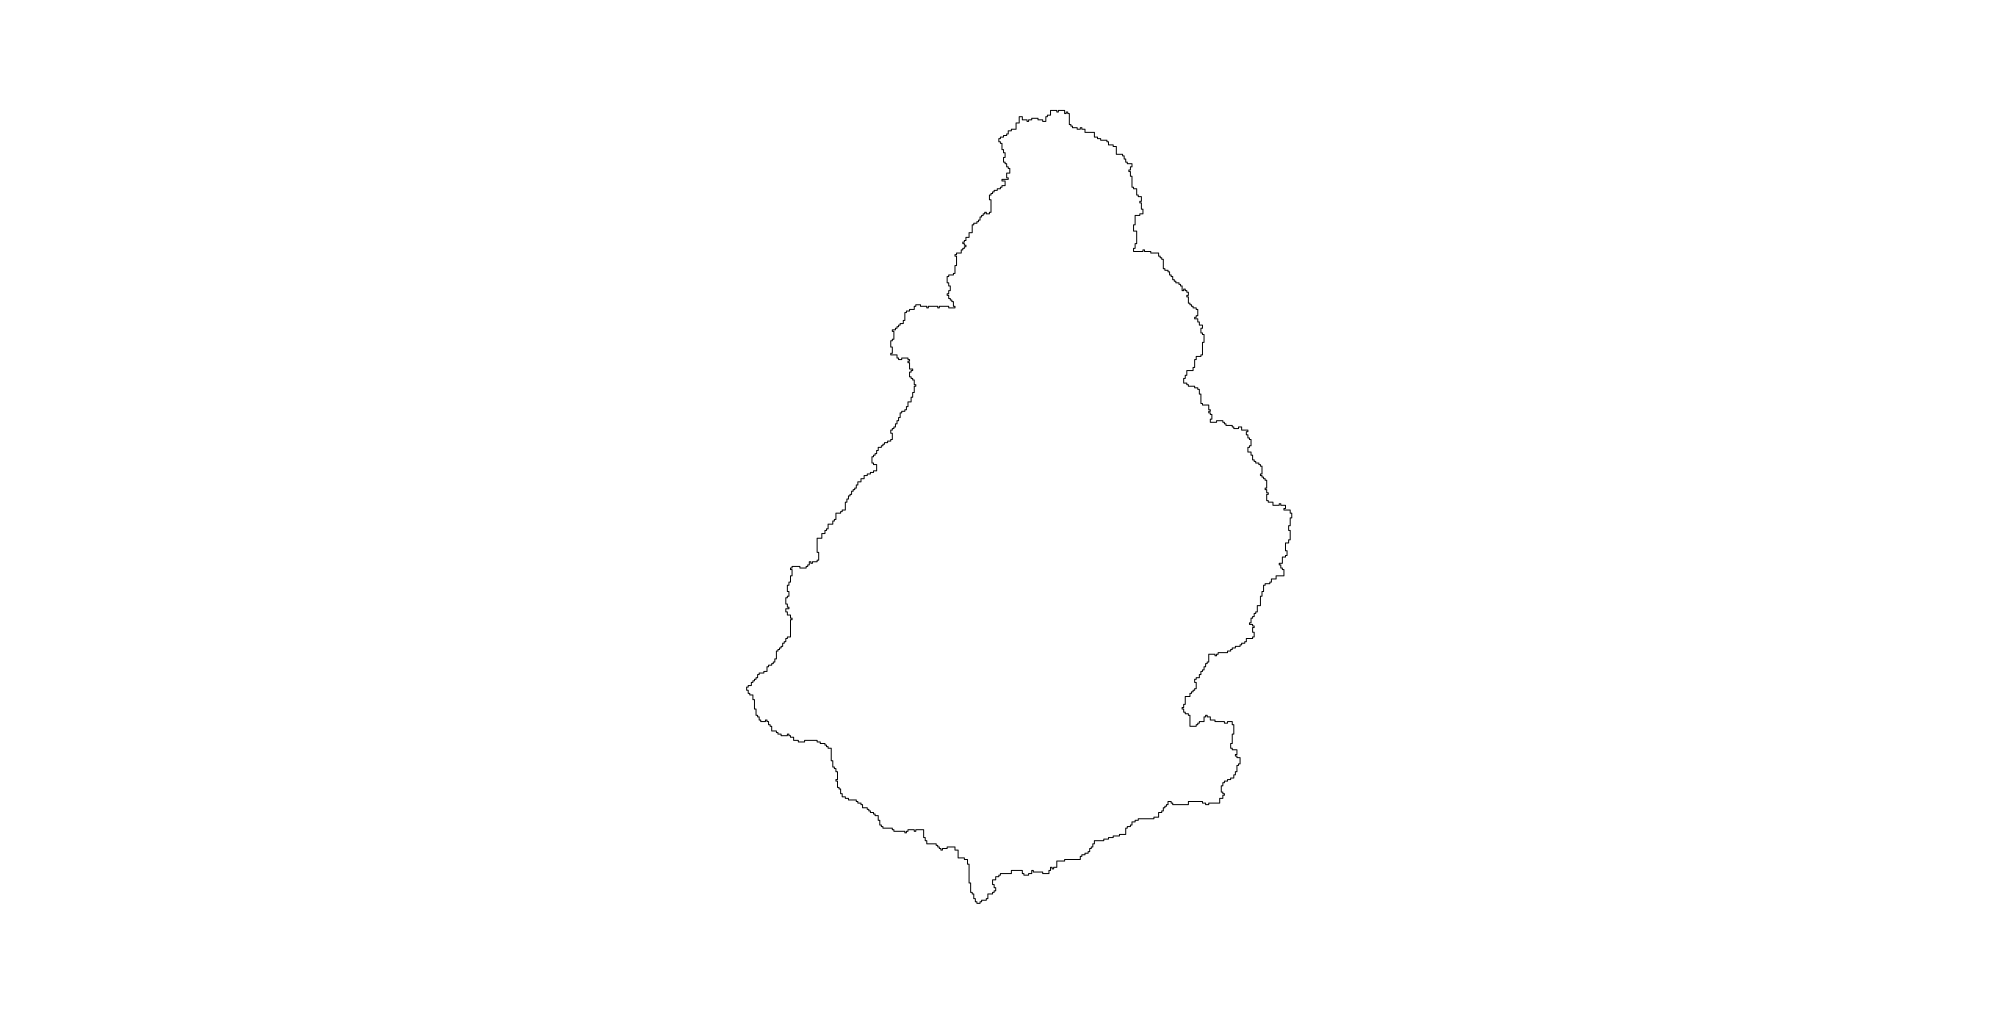
\includegraphics[width=0.50000\textwidth]{cuenca extraida.png}
\caption{Cuenca del río Guayubín\label{cuencavectorial}}
\end{figure}

\begin{figure}
\centering
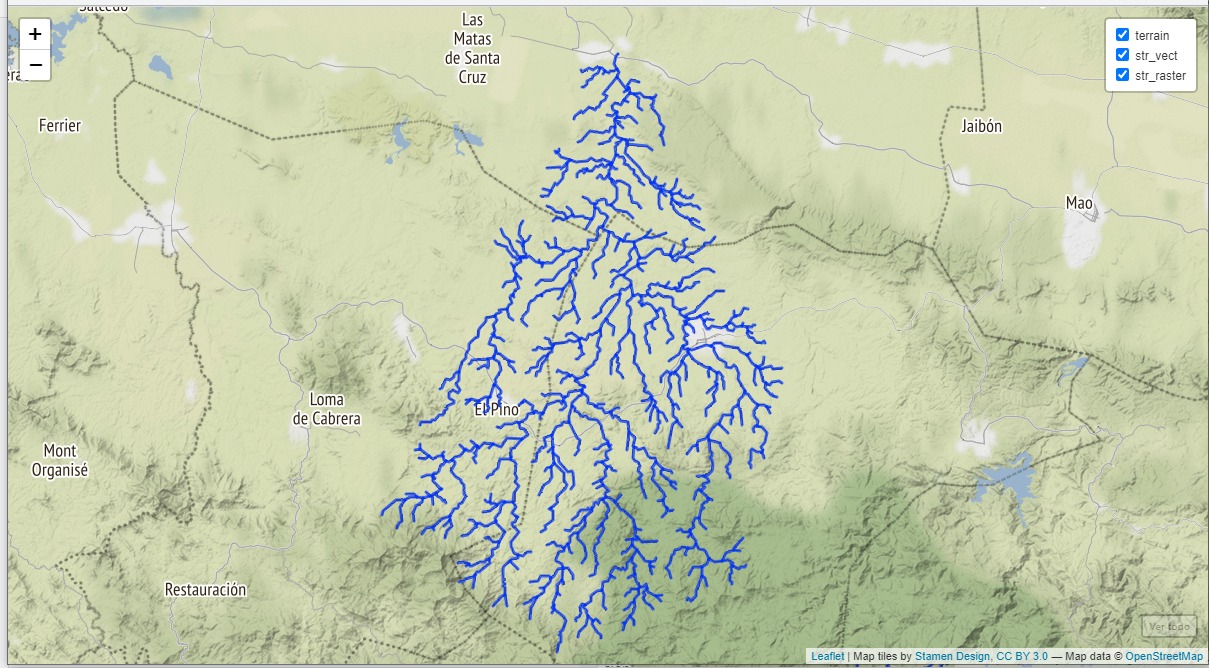
\includegraphics[width=0.70000\textwidth]{red de drenaje extraida.png}
\caption{Red de drenaje del río Guayubín\label{red de drenaje extraida}}
\end{figure}

\subsection{Orden de red analisis
hortoniano}\label{orden-de-red-analisis-hortoniano}

El orden de red de cada tramo fluvial de la cuenca según Strahler,
indicó que el orden de red máximo (5) y el minimo (1). (ver
figura\ref{unica}, y figura\ref{subcuencas}). Las estadísticas por orden
de red según la clasificación de Strahler, obtenidas con
\texttt{r.stream.stats} indican que el numero total de redes en la
cuenca es de 367, tambien se obtuvieron el total longitud por ordenes de
red resultando en 693.61 km (ver tabla \ref{tab:estadisticaor}). De la
misma manera se genero el dato de la razon de bifurcacion para la red
basada en el coeficiente de regresion es de 4.1, tambien se obtuvieron
resultados de razon de bifurcacion para cada orden de red, para el redes
de orden 1 (4.7), de orden 2 (3.6), orden 3 (4.3), para los de orden 4
(4), y para los de orden 5 (0), las otras estadisticas estan detalladas
en la tabla\ref{tab:estadisticaor} y sus derivadas en esta figura (ver
figura\ref{grafnumero}). Como se observa en las tablas
\ref{tab:regresionc} y ref\{tab:estandard\}, las razones de bifurcacion
se obtuvieron razones de bifurcacion con criterios distintos. Otras
estadisticas como la longitud promedio y area promedio para cada orden
de red estas detalladas en la tabla \ref{promo}. Tambien, se obtuvieron
las estadisticas de la desviacion estandar de ares y longitudes por
orden de red, ver tabla \ref{estad}. De igual manera se generaron las
estadisticas de los parametros hidrgograficos (numero de orden, longitud
y areas), segun el orden de red (ver tabla \ref{parh}). En tabla
\ref{razones}, se presentan los valores resultantes para la razon de
bifurcacion.

\begin{figure}
\centering
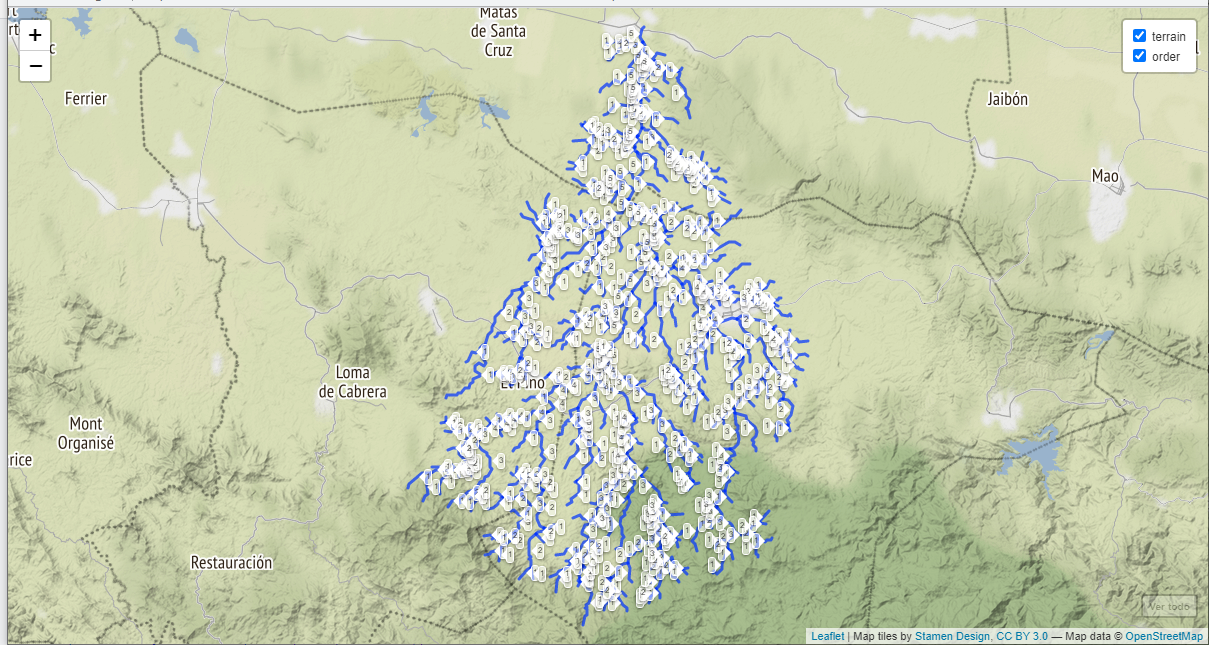
\includegraphics[width=1.00000\textwidth]{ordenes de red.png}
\caption{Ordenes de red del río Guayubín con simbología
única\label{unica}}
\end{figure}

\begin{figure}
\centering
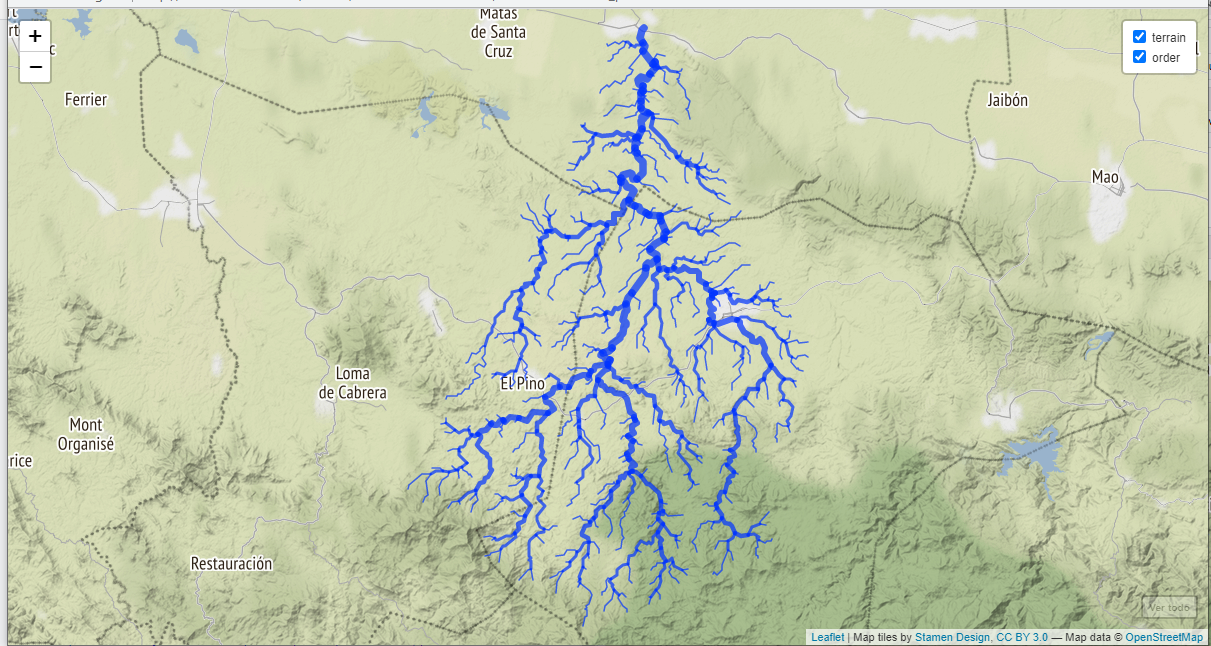
\includegraphics[width=0.80000\textwidth]{orden de red mapa 2.png}
\caption{Ordenes de red del río Guayubín con simbología aplicando grosor
según su orden\label{grosor}}
\end{figure}

\begin{figure}
\centering
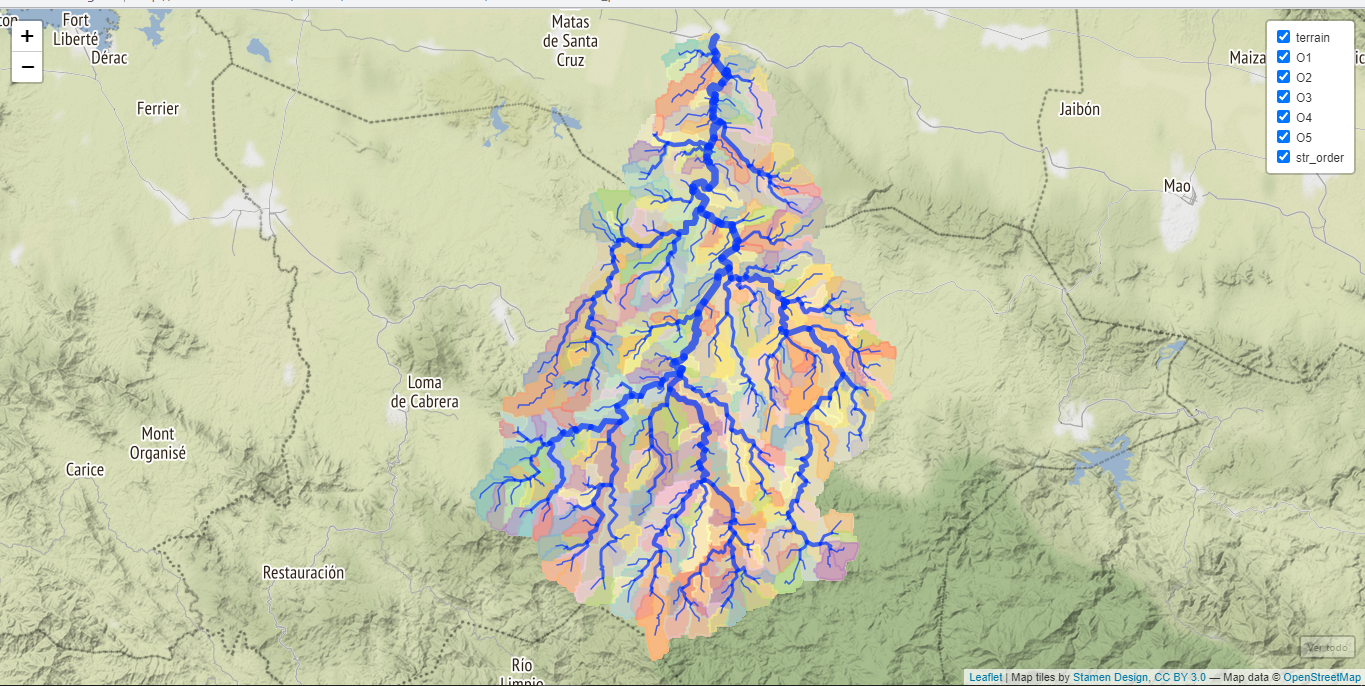
\includegraphics[width=0.70000\textwidth]{cuencas delimitadas y ordenes de red.png}
\caption{Subcuencas y ordenes de red del río Guayubín\label{subcuencas}}
\end{figure}

\begin{figure}
\centering
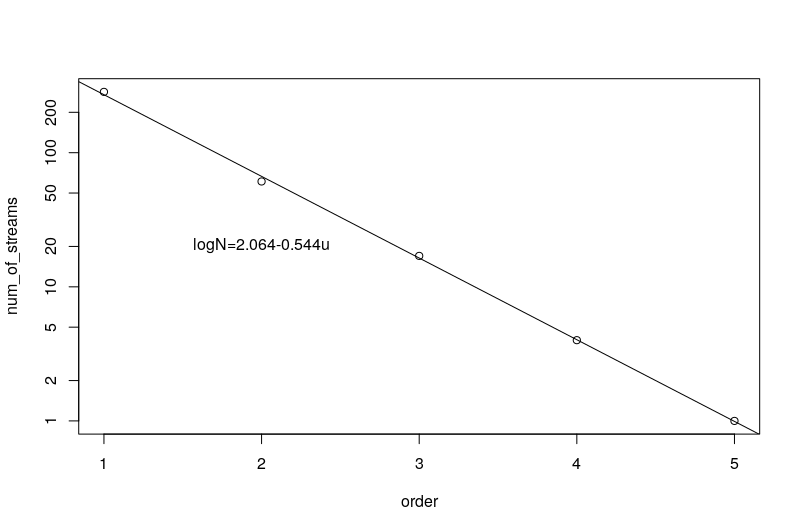
\includegraphics[width=0.80000\textwidth]{Numero de red segun su orden.png}
\caption{Número de redes según su orden y Razón de
bifurcación\label{grafnumero}}
\end{figure}

\begin{longtable}[]{@{}cccccc@{}}
\caption{\label{tab:estadisticaor} Estadisticas de los ordenes de red
del rio Guayubin}\tabularnewline
\toprule
Max order & Tot.N.str. & Tot.str.len. & Tot.area. & Dr.dens. &
Str.freq.\tabularnewline
\midrule
\endfirsthead
\toprule
Max order & Tot.N.str. & Tot.str.len. & Tot.area. & Dr.dens. &
Str.freq.\tabularnewline
\midrule
\endhead
(num) & (num) & (km) & (km\textsuperscript{2}) &
(km/km\textsuperscript{2}) & (num/km\textsuperscript{2})\tabularnewline
5 & 367 & 693.6069 & 773.2235 & 0.8970 & 0.4746\tabularnewline
\bottomrule
\end{longtable}

\begin{longtable}[]{@{}ccccc@{}}
\caption{\label{tab:regresionc} Razones de cursos basados en el
coeficiente de regresion}\tabularnewline
\toprule
Bif.rt. & Len.rt. & Area.rt. & Slo.rt. & Grd.rt.\tabularnewline
\midrule
\endfirsthead
\toprule
Bif.rt. & Len.rt. & Area.rt. & Slo.rt. & Grd.rt.\tabularnewline
\midrule
\endhead
4.0643 & 2.2928 & 4.5845 & 1.4798 & 1.8338\tabularnewline
\bottomrule
\end{longtable}

\begin{longtable}[]{@{}ccccc@{}}
\caption{\label{estandard} Relaciones de flujo promediadas con
desviaciones estándar}\tabularnewline
\toprule
Bif.rt. & Len.rt. & Area.rt. & Slo.rt. & Grd.rt.\tabularnewline
\midrule
\endfirsthead
\toprule
Bif.rt. & Len.rt. & Area.rt. & Slo.rt. & Grd.rt.\tabularnewline
\midrule
\endhead
4.1235 & 2.3822 & 3.3126 & 1.4938 & 1.9010\tabularnewline
0.4476 & 0.6025 & 2.2153 & 0.0960 & 0.5050\tabularnewline
\bottomrule
\end{longtable}

\begin{longtable}[]{@{}cccccc@{}}
\caption{\label{promo} Variables promediadas para cada orden de
red}\tabularnewline
\toprule
\begin{minipage}[b]{0.08\columnwidth}\centering\strut
Order num\strut
\end{minipage} & \begin{minipage}[b]{0.11\columnwidth}\centering\strut
Avg.len (km)\strut
\end{minipage} & \begin{minipage}[b]{0.25\columnwidth}\centering\strut
Avg.ar (km\textsuperscript{2})\strut
\end{minipage} & \begin{minipage}[b]{0.11\columnwidth}\centering\strut
Avg.sl (m/m)\strut
\end{minipage} & \begin{minipage}[b]{0.14\columnwidth}\centering\strut
Avg.grad. (m/m)\strut
\end{minipage} & \begin{minipage}[b]{0.13\columnwidth}\centering\strut
Avg.el.dif (m)\strut
\end{minipage}\tabularnewline
\midrule
\endfirsthead
\toprule
\begin{minipage}[b]{0.08\columnwidth}\centering\strut
Order num\strut
\end{minipage} & \begin{minipage}[b]{0.11\columnwidth}\centering\strut
Avg.len (km)\strut
\end{minipage} & \begin{minipage}[b]{0.25\columnwidth}\centering\strut
Avg.ar (km\textsuperscript{2})\strut
\end{minipage} & \begin{minipage}[b]{0.11\columnwidth}\centering\strut
Avg.sl (m/m)\strut
\end{minipage} & \begin{minipage}[b]{0.14\columnwidth}\centering\strut
Avg.grad. (m/m)\strut
\end{minipage} & \begin{minipage}[b]{0.13\columnwidth}\centering\strut
Avg.el.dif (m)\strut
\end{minipage}\tabularnewline
\midrule
\endhead
\begin{minipage}[t]{0.08\columnwidth}\centering\strut
1\strut
\end{minipage} & \begin{minipage}[t]{0.11\columnwidth}\centering\strut
1.2435\strut
\end{minipage} & \begin{minipage}[t]{0.25\columnwidth}\centering\strut
1.7188\strut
\end{minipage} & \begin{minipage}[t]{0.11\columnwidth}\centering\strut
0.0367\strut
\end{minipage} & \begin{minipage}[t]{0.14\columnwidth}\centering\strut
0.0296\strut
\end{minipage} & \begin{minipage}[t]{0.13\columnwidth}\centering\strut
37.4437\strut
\end{minipage}\tabularnewline
\begin{minipage}[t]{0.08\columnwidth}\centering\strut
2\strut
\end{minipage} & \begin{minipage}[t]{0.11\columnwidth}\centering\strut
2.4743\strut
\end{minipage} & \begin{minipage}[t]{0.25\columnwidth}\centering\strut
7.2904\strut
\end{minipage} & \begin{minipage}[t]{0.11\columnwidth}\centering\strut
0.0246\strut
\end{minipage} & \begin{minipage}[t]{0.14\columnwidth}\centering\strut
0.0201\strut
\end{minipage} & \begin{minipage}[t]{0.13\columnwidth}\centering\strut
49.0820\strut
\end{minipage}\tabularnewline
\begin{minipage}[t]{0.08\columnwidth}\centering\strut
3\strut
\end{minipage} & \begin{minipage}[t]{0.11\columnwidth}\centering\strut
6.2881\strut
\end{minipage} & \begin{minipage}[t]{0.25\columnwidth}\centering\strut
31.7328\strut
\end{minipage} & \begin{minipage}[t]{0.11\columnwidth}\centering\strut
0.0165\strut
\end{minipage} & \begin{minipage}[t]{0.14\columnwidth}\centering\strut
0.0113\strut
\end{minipage} & \begin{minipage}[t]{0.13\columnwidth}\centering\strut
85.1765\strut
\end{minipage}\tabularnewline
\begin{minipage}[t]{0.08\columnwidth}\centering\strut
4\strut
\end{minipage} & \begin{minipage}[t]{0.11\columnwidth}\centering\strut
11.5356\strut
\end{minipage} & \begin{minipage}[t]{0.25\columnwidth}\centering\strut
147.7492\strut
\end{minipage} & \begin{minipage}[t]{0.11\columnwidth}\centering\strut
0.0120\strut
\end{minipage} & \begin{minipage}[t]{0.14\columnwidth}\centering\strut
0.0066\strut
\end{minipage} & \begin{minipage}[t]{0.13\columnwidth}\centering\strut
80.0000\strut
\end{minipage}\tabularnewline
\begin{minipage}[t]{0.08\columnwidth}\centering\strut
5\strut
\end{minipage} & \begin{minipage}[t]{0.11\columnwidth}\centering\strut
36.4888\strut
\end{minipage} & \begin{minipage}[t]{0.25\columnwidth}\centering\strut
773.2235\strut
\end{minipage} & \begin{minipage}[t]{0.11\columnwidth}\centering\strut
0.0074\strut
\end{minipage} & \begin{minipage}[t]{0.14\columnwidth}\centering\strut
0.0025\strut
\end{minipage} & \begin{minipage}[t]{0.13\columnwidth}\centering\strut
91.0000\strut
\end{minipage}\tabularnewline
\bottomrule
\end{longtable}

\begin{longtable}[]{@{}cccccc@{}}
\caption{\label{estad} Desviacion estandar para las estadisticas segun
orden de red}\tabularnewline
\toprule
\begin{minipage}[b]{0.08\columnwidth}\centering\strut
Order num\strut
\end{minipage} & \begin{minipage}[b]{0.11\columnwidth}\centering\strut
Std.len (km)\strut
\end{minipage} & \begin{minipage}[b]{0.26\columnwidth}\centering\strut
Std.ar (km\textsuperscript{2})\strut
\end{minipage} & \begin{minipage}[b]{0.11\columnwidth}\centering\strut
Std.sl (m/m)\strut
\end{minipage} & \begin{minipage}[b]{0.14\columnwidth}\centering\strut
Std.grad. (m/m)\strut
\end{minipage} & \begin{minipage}[b]{0.13\columnwidth}\centering\strut
Std.el.dif (m)\strut
\end{minipage}\tabularnewline
\midrule
\endfirsthead
\toprule
\begin{minipage}[b]{0.08\columnwidth}\centering\strut
Order num\strut
\end{minipage} & \begin{minipage}[b]{0.11\columnwidth}\centering\strut
Std.len (km)\strut
\end{minipage} & \begin{minipage}[b]{0.26\columnwidth}\centering\strut
Std.ar (km\textsuperscript{2})\strut
\end{minipage} & \begin{minipage}[b]{0.11\columnwidth}\centering\strut
Std.sl (m/m)\strut
\end{minipage} & \begin{minipage}[b]{0.14\columnwidth}\centering\strut
Std.grad. (m/m)\strut
\end{minipage} & \begin{minipage}[b]{0.13\columnwidth}\centering\strut
Std.el.dif (m)\strut
\end{minipage}\tabularnewline
\midrule
\endhead
\begin{minipage}[t]{0.08\columnwidth}\centering\strut
1\strut
\end{minipage} & \begin{minipage}[t]{0.11\columnwidth}\centering\strut
1.0274\strut
\end{minipage} & \begin{minipage}[t]{0.26\columnwidth}\centering\strut
1.0955\strut
\end{minipage} & \begin{minipage}[t]{0.11\columnwidth}\centering\strut
0.0379\strut
\end{minipage} & \begin{minipage}[t]{0.14\columnwidth}\centering\strut
0.0324\strut
\end{minipage} & \begin{minipage}[t]{0.13\columnwidth}\centering\strut
52.7742\strut
\end{minipage}\tabularnewline
\begin{minipage}[t]{0.08\columnwidth}\centering\strut
2\strut
\end{minipage} & \begin{minipage}[t]{0.11\columnwidth}\centering\strut
1.9695\strut
\end{minipage} & \begin{minipage}[t]{0.26\columnwidth}\centering\strut
4.4097\strut
\end{minipage} & \begin{minipage}[t]{0.11\columnwidth}\centering\strut
0.0215\strut
\end{minipage} & \begin{minipage}[t]{0.14\columnwidth}\centering\strut
0.0194\strut
\end{minipage} & \begin{minipage}[t]{0.13\columnwidth}\centering\strut
52.5830\strut
\end{minipage}\tabularnewline
\begin{minipage}[t]{0.08\columnwidth}\centering\strut
3\strut
\end{minipage} & \begin{minipage}[t]{0.11\columnwidth}\centering\strut
5.0992\strut
\end{minipage} & \begin{minipage}[t]{0.26\columnwidth}\centering\strut
19.0637\strut
\end{minipage} & \begin{minipage}[t]{0.11\columnwidth}\centering\strut
0.0092\strut
\end{minipage} & \begin{minipage}[t]{0.14\columnwidth}\centering\strut
0.0077\strut
\end{minipage} & \begin{minipage}[t]{0.13\columnwidth}\centering\strut
93.4085\strut
\end{minipage}\tabularnewline
\begin{minipage}[t]{0.08\columnwidth}\centering\strut
4\strut
\end{minipage} & \begin{minipage}[t]{0.11\columnwidth}\centering\strut
5.8247\strut
\end{minipage} & \begin{minipage}[t]{0.26\columnwidth}\centering\strut
44.3177\strut
\end{minipage} & \begin{minipage}[t]{0.11\columnwidth}\centering\strut
0.0041\strut
\end{minipage} & \begin{minipage}[t]{0.14\columnwidth}\centering\strut
0.0032\strut
\end{minipage} & \begin{minipage}[t]{0.13\columnwidth}\centering\strut
57.0789\strut
\end{minipage}\tabularnewline
\begin{minipage}[t]{0.08\columnwidth}\centering\strut
5\strut
\end{minipage} & \begin{minipage}[t]{0.11\columnwidth}\centering\strut
-0.0000\strut
\end{minipage} & \begin{minipage}[t]{0.26\columnwidth}\centering\strut
0.0000\strut
\end{minipage} & \begin{minipage}[t]{0.11\columnwidth}\centering\strut
0.0000\strut
\end{minipage} & \begin{minipage}[t]{0.14\columnwidth}\centering\strut
0.0000\strut
\end{minipage} & \begin{minipage}[t]{0.13\columnwidth}\centering\strut
0.0000\strut
\end{minipage}\tabularnewline
\bottomrule
\end{longtable}

\begin{longtable}[]{@{}cccc@{}}
\caption{\label{parh} Estadisticas de parametros hidrgograficos segun el
orden de red}\tabularnewline
\toprule
Order & N.streams & Tot.len (km) & Tot.area
(km\textsuperscript{2})\tabularnewline
\midrule
\endfirsthead
\toprule
Order & N.streams & Tot.len (km) & Tot.area
(km\textsuperscript{2})\tabularnewline
\midrule
\endhead
1 & 284 & 353.1463 & 488.1383\tabularnewline
2 & 61 & 150.9325 & 444.7173\tabularnewline
3 & 17 & 106.8969 & 539.4576\tabularnewline
4 & 4 & 46.1425 & 590.9969\tabularnewline
5 & 1 & 36.4888 & 773.2235\tabularnewline
\bottomrule
\end{longtable}

\begin{longtable}[]{@{}cccccccc@{}}
\caption{\label{razones} Razones de los parametros hidrograficos segun
su orden de red}\tabularnewline
\toprule
Order & Bif.rt. & Len.rt. & Area.rt. & Slo.rt. & Grd.rt. & d.dens. &
str.freq.\tabularnewline
\midrule
\endfirsthead
\toprule
Order & Bif.rt. & Len.rt. & Area.rt. & Slo.rt. & Grd.rt. & d.dens. &
str.freq.\tabularnewline
\midrule
\endhead
1 & 4.6557 & 1.9898 & 0.0000 & 1.4930 & 1.4748 & 0.7235 &
0.5818\tabularnewline
2 & 3.5882 & 2.5413 & 4.2416 & 1.4930 & 1.7757 & 0.3394 &
0.1372\tabularnewline
3 & 4.2500 & 1.8345 & 4.3527 & 1.3771 & 1.7207 & 0.1982 &
0.0315\tabularnewline
4 & 4.0000 & 3.1631 & 4.6560 & 1.6122 & 2.6327 & 0.0781 &
0.0068\tabularnewline
5 & 0.0000 & 0.0000 & 5.2334 & 0.0000 & 0.0000 & 0.0472 &
0.0013\tabularnewline
\bottomrule
\end{longtable}

\subsection{Índices de concavidad y perfiles
longitudinales}\label{uxedndices-de-concavidad-y-perfiles-longitudinales}

Con la función \texttt{LfpNetwork} se obtuvieron los cursos más largos
de la red de drenaje, siendo un total de 60 cursos. De los cuales los
cursos 30, 48, 52, 55 y 56 (0.59; 0.51; 0.51; 0.54; y 0.47,
respectivamente), presentaron los mas altos indices de concavidad;
siendo el curso 30 el poseedor del indice de concavidad mas alto de
todos los cursos. Mientras que los cursos de agua 15, 16, 23 y 38
presentaron valores menores a 0.03, poseyendo los valores as bajos de
todos los cursos (ver figura\ref{lfpnet}, \ref{plongitudinal} y
\ref{indicec}).

\begin{figure}
\centering
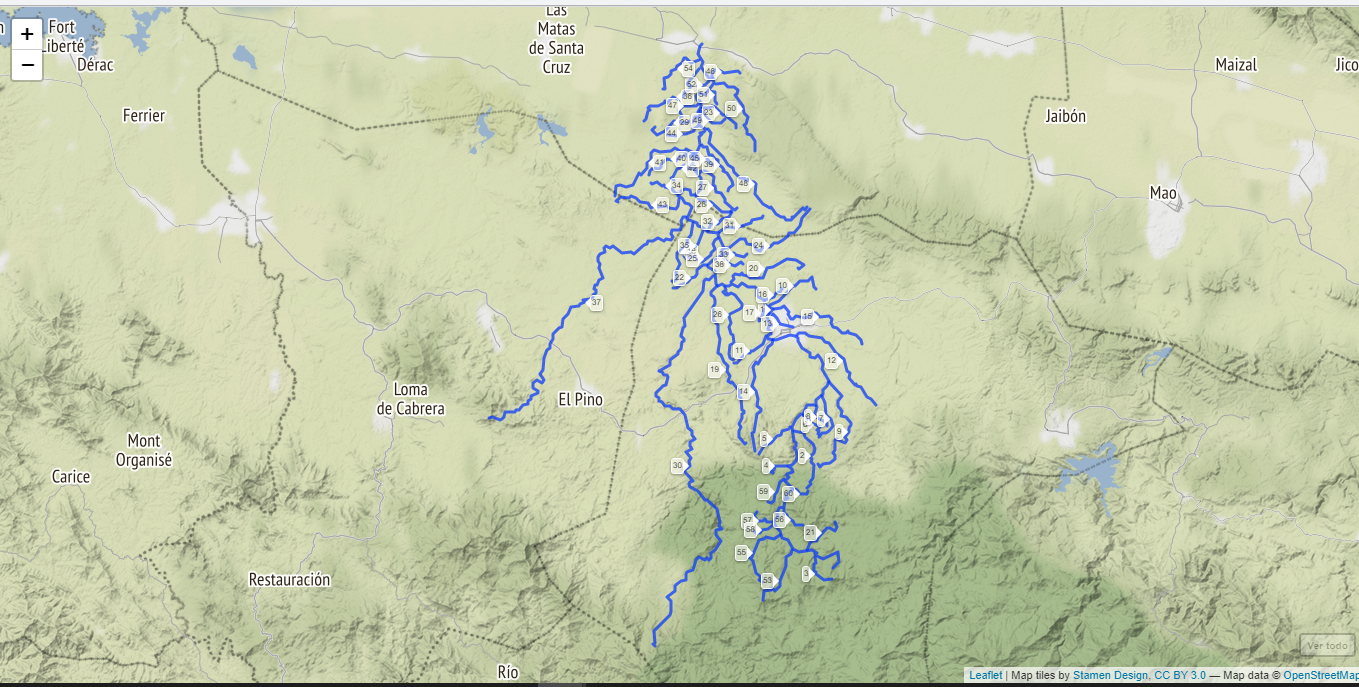
\includegraphics[width=1.00000\textwidth]{cursos mas largos.png}
\caption{Cursos fluviales mas largos de la cuenca del río
Guayubín\label{lfpnet}}
\end{figure}

\begin{figure}
\centering
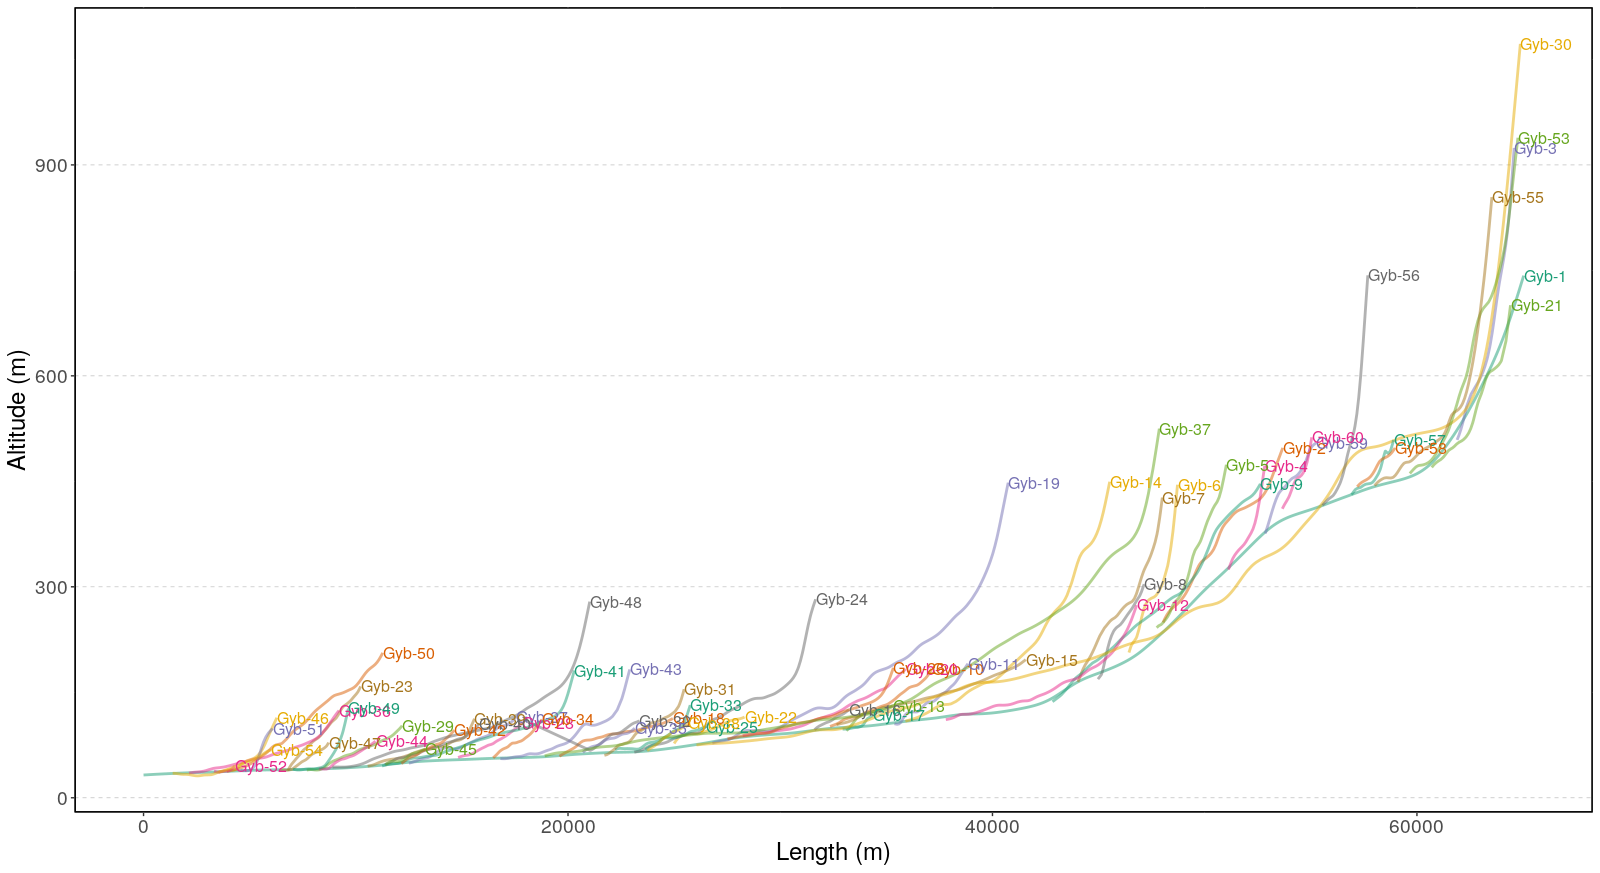
\includegraphics[width=1.00000\textwidth]{perfiles longitudinales.png}
\caption{Perfiles longitudinales de los cursos más largos en la cuenca
del río Guayubín\label{plongitudinal}}
\end{figure}

\begin{figure}
\centering
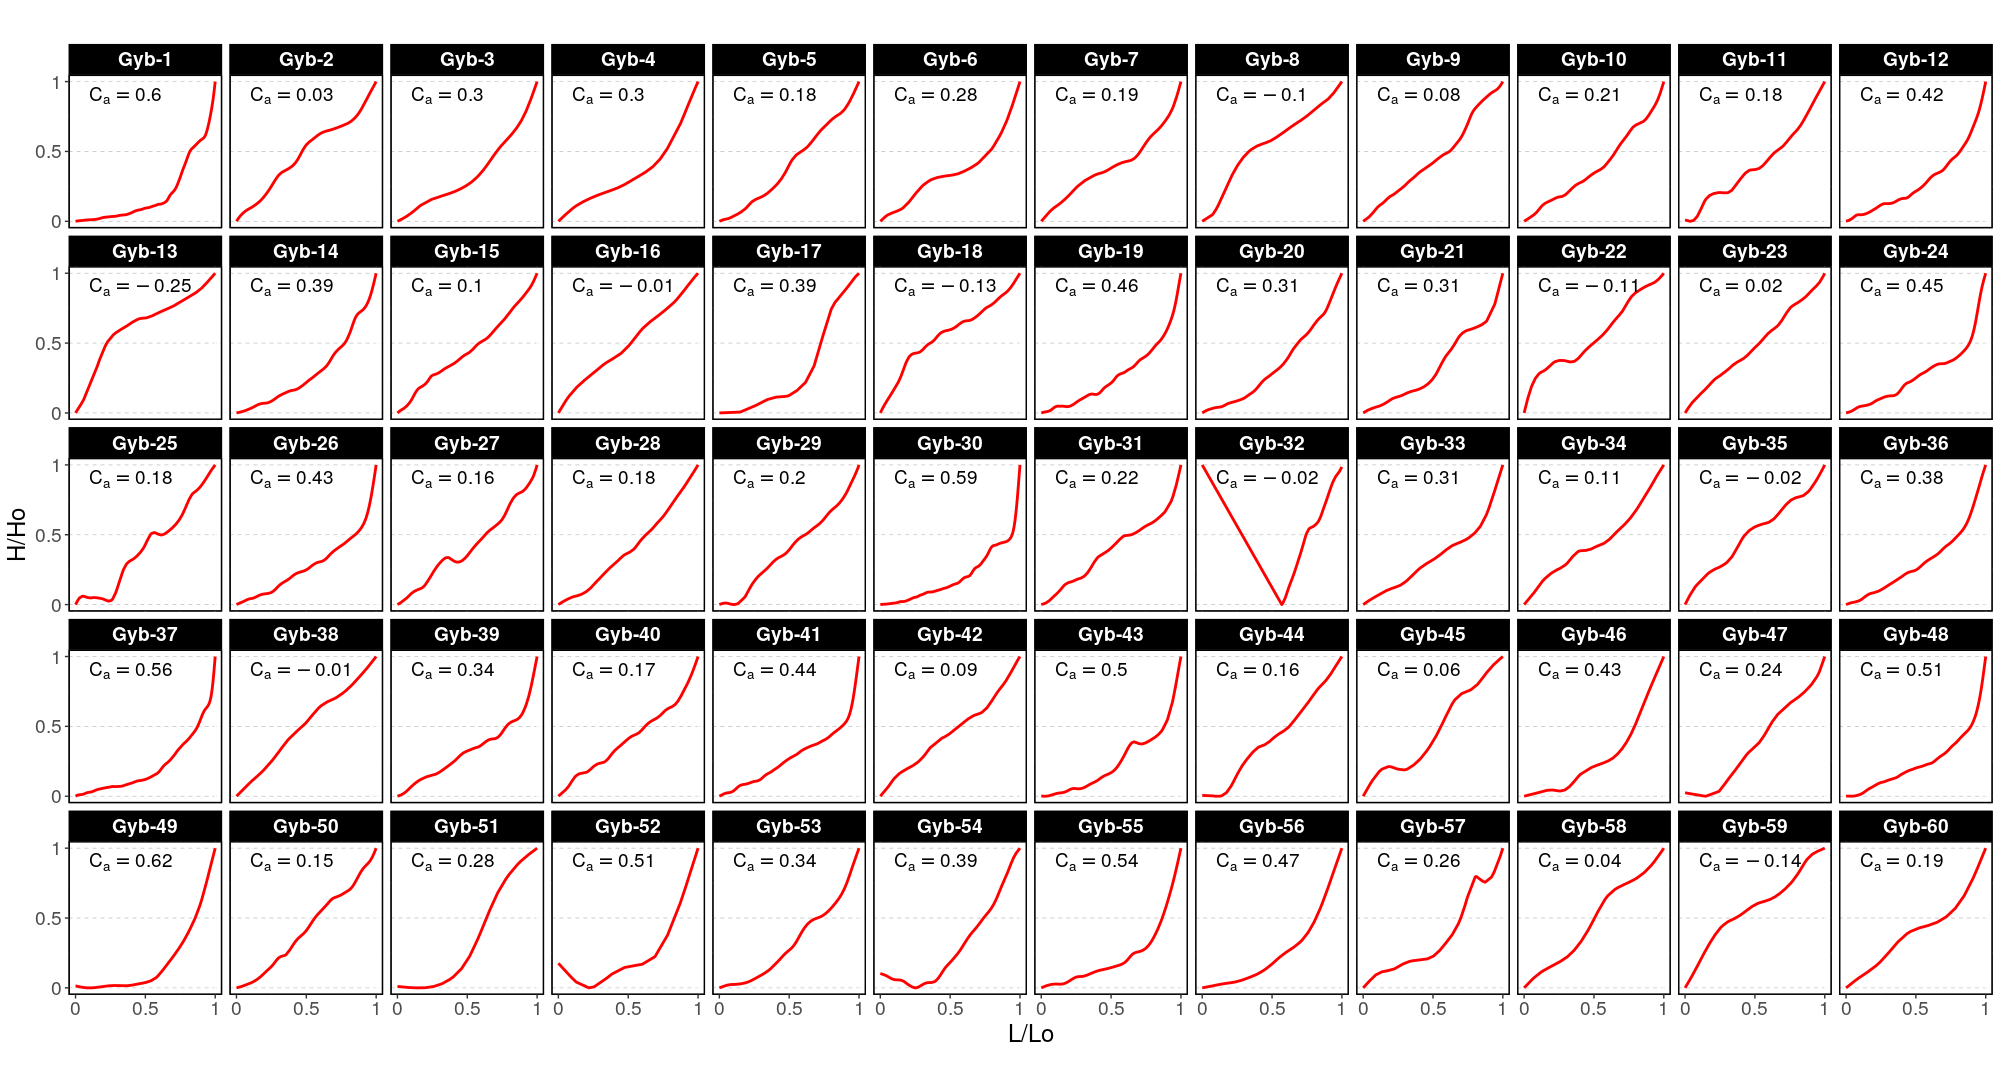
\includegraphics[width=1.00000\textwidth]{Indices de concavidad.png}
\caption{Perfiles longitudinales e índices de concavidad de los cursos
más largos en la cuenca del río Guayubín\label{indicec}}
\end{figure}

\subsection{Morfometría de cuenca}\label{morfometruxeda-de-cuenca}

Los parametros morfometricos obtenidos con \texttt{r.basin}, indicaron
que la elevacion minima en la cuenca del rio Guayubin fue 30.97 mslm y
la maxima fue 1396.73 mslm, mientras la diferencia de elevacion obtenida
de los claculos fue de 1365.76 m. Asi mismo, se produjo el parametro de
elevacion media (276.70). El parametro de coeficiente de compacidad
obtenido fue de 4.9. El curso mas largo de la red de drenaje o curso
principal en la cuenca producido por \texttt{r.basin} presento una
longitud de 61.96 km. El resto de los parametros obtenidos estan
resumidos en la tabla \ref{tab:parametrosm}.

\begin{figure}
\centering
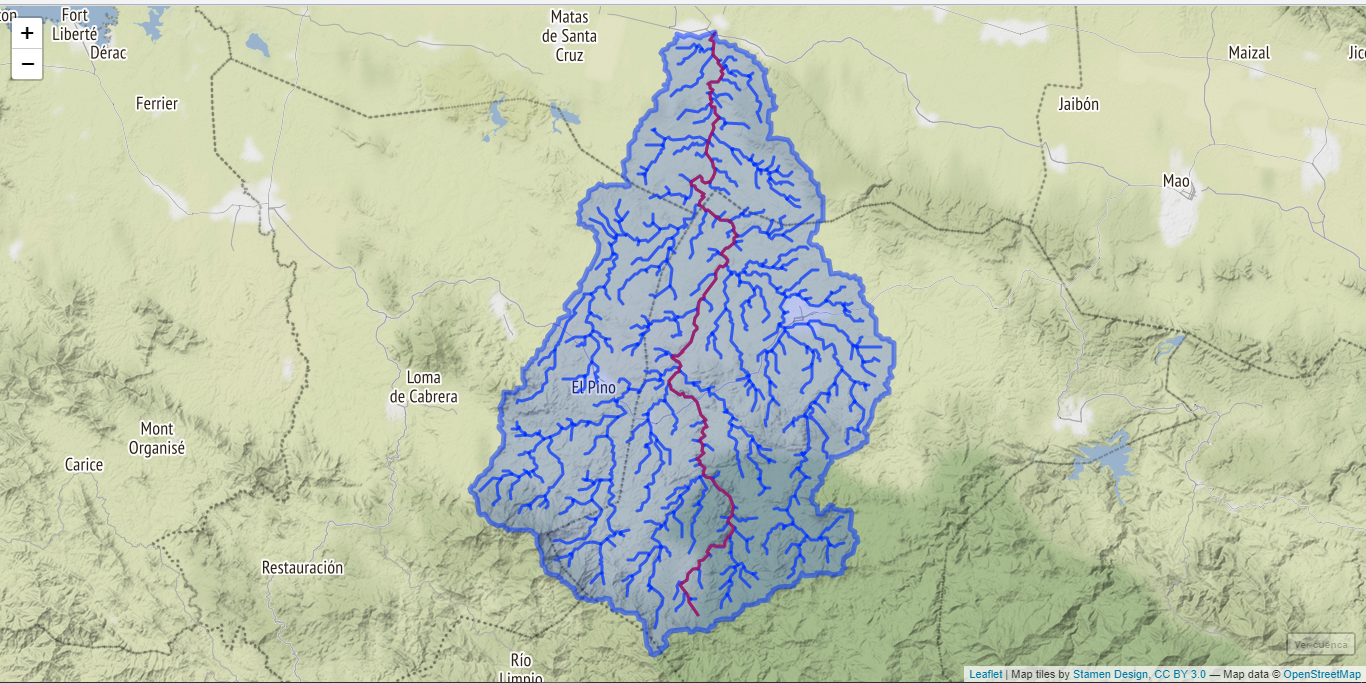
\includegraphics[width=0.60000\textwidth]{cuenca-red de drenaje-curso mas largo.png}
\caption{Cuenca del río Guayubín con su red de drenaje y su curso más
largo\label{vectoresrbasin}}
\end{figure}

\begin{longtable}[]{@{}cc@{}}
\caption{\label{tab:parametrosm}Parámetros morfométricos de la cuenca
del río Guayubín.}\tabularnewline
\toprule
\begin{minipage}[b]{0.65\columnwidth}\centering\strut
Parámetros\strut
\end{minipage} & \begin{minipage}[b]{0.29\columnwidth}\centering\strut
Valores\strut
\end{minipage}\tabularnewline
\midrule
\endfirsthead
\toprule
\begin{minipage}[b]{0.65\columnwidth}\centering\strut
Parámetros\strut
\end{minipage} & \begin{minipage}[b]{0.29\columnwidth}\centering\strut
Valores\strut
\end{minipage}\tabularnewline
\midrule
\endhead
\begin{minipage}[t]{0.65\columnwidth}\centering\strut
Easting Centroid of basin\strut
\end{minipage} & \begin{minipage}[t]{0.29\columnwidth}\centering\strut
246465.00\strut
\end{minipage}\tabularnewline
\begin{minipage}[t]{0.65\columnwidth}\centering\strut
Northing Centroid of basin\strut
\end{minipage} & \begin{minipage}[t]{0.29\columnwidth}\centering\strut
2151675.00\strut
\end{minipage}\tabularnewline
\begin{minipage}[t]{0.65\columnwidth}\centering\strut
Rectangle containing basin N-W\strut
\end{minipage} & \begin{minipage}[t]{0.29\columnwidth}\centering\strut
(`230220', `2175930')\strut
\end{minipage}\tabularnewline
\begin{minipage}[t]{0.65\columnwidth}\centering\strut
Rectangle containing basin S-E\strut
\end{minipage} & \begin{minipage}[t]{0.29\columnwidth}\centering\strut
(`261000', `2131290')\strut
\end{minipage}\tabularnewline
\begin{minipage}[t]{0.65\columnwidth}\centering\strut
Area of basin {[}km\textsuperscript{2}{]}\strut
\end{minipage} & \begin{minipage}[t]{0.29\columnwidth}\centering\strut
773.5631625\strut
\end{minipage}\tabularnewline
\begin{minipage}[t]{0.65\columnwidth}\centering\strut
Perimeter of basin {[}km{]}\strut
\end{minipage} & \begin{minipage}[t]{0.29\columnwidth}\centering\strut
156.122652506552\strut
\end{minipage}\tabularnewline
\begin{minipage}[t]{0.65\columnwidth}\centering\strut
Max Elevation {[}m s.l.m.{]}\strut
\end{minipage} & \begin{minipage}[t]{0.29\columnwidth}\centering\strut
1396.72540740785\strut
\end{minipage}\tabularnewline
\begin{minipage}[t]{0.65\columnwidth}\centering\strut
Min Elevation {[}m s.l.m.{]}\strut
\end{minipage} & \begin{minipage}[t]{0.29\columnwidth}\centering\strut
30.9651954818271\strut
\end{minipage}\tabularnewline
\begin{minipage}[t]{0.65\columnwidth}\centering\strut
Elevation Difference {[}m{]}\strut
\end{minipage} & \begin{minipage}[t]{0.29\columnwidth}\centering\strut
1365.760211926023\strut
\end{minipage}\tabularnewline
\begin{minipage}[t]{0.65\columnwidth}\centering\strut
Mean Elevation\strut
\end{minipage} & \begin{minipage}[t]{0.29\columnwidth}\centering\strut
276.7019\strut
\end{minipage}\tabularnewline
\begin{minipage}[t]{0.65\columnwidth}\centering\strut
Mean Slope\strut
\end{minipage} & \begin{minipage}[t]{0.29\columnwidth}\centering\strut
5.17\strut
\end{minipage}\tabularnewline
\begin{minipage}[t]{0.65\columnwidth}\centering\strut
Length of Directing Vector {[}km{]}\strut
\end{minipage} & \begin{minipage}[t]{0.29\columnwidth}\centering\strut
24.460893544594807\strut
\end{minipage}\tabularnewline
\begin{minipage}[t]{0.65\columnwidth}\centering\strut
Prevalent Orientation {[}degree from north, counterclockwise{]}\strut
\end{minipage} & \begin{minipage}[t]{0.29\columnwidth}\centering\strut
1.4935760627096282\strut
\end{minipage}\tabularnewline
\begin{minipage}[t]{0.65\columnwidth}\centering\strut
Compactness Coefficient\strut
\end{minipage} & \begin{minipage}[t]{0.29\columnwidth}\centering\strut
4.974655054098116\strut
\end{minipage}\tabularnewline
\begin{minipage}[t]{0.65\columnwidth}\centering\strut
Circularity Ratio\strut
\end{minipage} & \begin{minipage}[t]{0.29\columnwidth}\centering\strut
0.3988171279899944\strut
\end{minipage}\tabularnewline
\begin{minipage}[t]{0.65\columnwidth}\centering\strut
Topological Diameter\strut
\end{minipage} & \begin{minipage}[t]{0.29\columnwidth}\centering\strut
84.0\strut
\end{minipage}\tabularnewline
\begin{minipage}[t]{0.65\columnwidth}\centering\strut
Elongation Ratio\strut
\end{minipage} & \begin{minipage}[t]{0.29\columnwidth}\centering\strut
0.5064682945330589\strut
\end{minipage}\tabularnewline
\begin{minipage}[t]{0.65\columnwidth}\centering\strut
Shape Factor\strut
\end{minipage} & \begin{minipage}[t]{0.29\columnwidth}\centering\strut
12.483750895456415\strut
\end{minipage}\tabularnewline
\begin{minipage}[t]{0.65\columnwidth}\centering\strut
Concentration Time (Giandotti, 1934) {[}hr{]}\strut
\end{minipage} & \begin{minipage}[t]{0.29\columnwidth}\centering\strut
6.906840311938352\strut
\end{minipage}\tabularnewline
\begin{minipage}[t]{0.65\columnwidth}\centering\strut
Length of Mainchannel {[}km{]}\strut
\end{minipage} & \begin{minipage}[t]{0.29\columnwidth}\centering\strut
61.965603846\strut
\end{minipage}\tabularnewline
\begin{minipage}[t]{0.65\columnwidth}\centering\strut
Mean slope of mainchannel {[}percent{]}\strut
\end{minipage} & \begin{minipage}[t]{0.29\columnwidth}\centering\strut
1.9669190473941982\strut
\end{minipage}\tabularnewline
\begin{minipage}[t]{0.65\columnwidth}\centering\strut
Mean hillslope length {[}m{]}\strut
\end{minipage} & \begin{minipage}[t]{0.29\columnwidth}\centering\strut
250.4986\strut
\end{minipage}\tabularnewline
\begin{minipage}[t]{0.65\columnwidth}\centering\strut
Magnitudo\strut
\end{minipage} & \begin{minipage}[t]{0.29\columnwidth}\centering\strut
223.0\strut
\end{minipage}\tabularnewline
\begin{minipage}[t]{0.65\columnwidth}\centering\strut
Max order (Strahler)\strut
\end{minipage} & \begin{minipage}[t]{0.29\columnwidth}\centering\strut
5\strut
\end{minipage}\tabularnewline
\begin{minipage}[t]{0.65\columnwidth}\centering\strut
Number of streams\strut
\end{minipage} & \begin{minipage}[t]{0.29\columnwidth}\centering\strut
343\strut
\end{minipage}\tabularnewline
\begin{minipage}[t]{0.65\columnwidth}\centering\strut
Total Stream Length {[}km{]}\strut
\end{minipage} & \begin{minipage}[t]{0.29\columnwidth}\centering\strut
662.2185\strut
\end{minipage}\tabularnewline
\begin{minipage}[t]{0.65\columnwidth}\centering\strut
First order stream frequency\strut
\end{minipage} & \begin{minipage}[t]{0.29\columnwidth}\centering\strut
0.2882763952710843\strut
\end{minipage}\tabularnewline
\begin{minipage}[t]{0.65\columnwidth}\centering\strut
Drainage Density {[}km/km\textsuperscript{2}{]}\strut
\end{minipage} & \begin{minipage}[t]{0.29\columnwidth}\centering\strut
0.8560626101427108\strut
\end{minipage}\tabularnewline
\begin{minipage}[t]{0.65\columnwidth}\centering\strut
Bifurcation Ratio (Horton)\strut
\end{minipage} & \begin{minipage}[t]{0.29\columnwidth}\centering\strut
3.8876\strut
\end{minipage}\tabularnewline
\begin{minipage}[t]{0.65\columnwidth}\centering\strut
Length Ratio (Horton)\strut
\end{minipage} & \begin{minipage}[t]{0.29\columnwidth}\centering\strut
2.2966\strut
\end{minipage}\tabularnewline
\begin{minipage}[t]{0.65\columnwidth}\centering\strut
Area ratio (Horton)\strut
\end{minipage} & \begin{minipage}[t]{0.29\columnwidth}\centering\strut
4.3704\strut
\end{minipage}\tabularnewline
\begin{minipage}[t]{0.65\columnwidth}\centering\strut
Slope ratio (Horton)\strut
\end{minipage} & \begin{minipage}[t]{0.29\columnwidth}\centering\strut
1.4689\strut
\end{minipage}\tabularnewline
\bottomrule
\end{longtable}

Los estadisticas que se generaron sobre la curva y la integral
hipsométrica se obtuvieron 60 resultados para los cursos de agua
pertenecientes a la cuenca de orden 2. El valor minimo generado para la
integral hipsometrica fue 0.08 en el curso 43. En tanto, el valor maximo
para la integra fue de 0.48 en el curso 45 (ver tabla \ref{ihco2}). los
curso mas curvos fuero 37, 18 y 15. Ver figuras\ref{hypsob2} y
\ref{hypb2}.

En cuanto a las cursos de agua de las cuencas de orden 3, se produjeron
17 resultados, donde los cursos 8 (0.40), 11 (0.34), y 13 (0.33),
presentaron los valores de integral hipsometrica mas altos. Y los cursos
con los valores mas bajos de la integral hipsometrica fueron 4 (0.12), y
16 (0.06). Ver tabla \ref{ihco3}. y los cursos mas curvos obtenidos
fueron 5, 10, 17, y 18. Ver figuras \ref{hysob3} y \ref{hypb3}.

\begin{longtable}[]{@{}cc@{}}
\caption{\label{ihco2} Integral hipsométrica en las cuencas de orden
2}\tabularnewline
\toprule
Categoría & Integral hipsométrica\tabularnewline
\midrule
\endfirsthead
\toprule
Categoría & Integral hipsométrica\tabularnewline
\midrule
\endhead
1 & 0.23784092\tabularnewline
2 & 0.29691935\tabularnewline
3 & 0.31478851\tabularnewline
4 & 0.25845620\tabularnewline
5 & 0.18914104\tabularnewline
6 & 0.38449116\tabularnewline
7 & 0.25087104\tabularnewline
9 & 0.26943542\tabularnewline
10 & 0.19779399\tabularnewline
11 & 0.19287436\tabularnewline
12 & 0.17808813\tabularnewline
13 & 0.22437828\tabularnewline
14 & 0.40595651\tabularnewline
15 & 0.25477715\tabularnewline
16 & 0.19777159\tabularnewline
17 & 0.25313336\tabularnewline
18 & 0.22679929\tabularnewline
19 & 0.30597060\tabularnewline
20 & 0.30564285\tabularnewline
21 & 0.24773997\tabularnewline
22 & 0.21800099\tabularnewline
23 & 0.33229314\tabularnewline
24 & 0.40758028\tabularnewline
25 & 0.27096759\tabularnewline
26 & 0.17485732\tabularnewline
28 & 0.25721054\tabularnewline
29 & 0.27907973\tabularnewline
30 & 0.23545394\tabularnewline
32 & 0.24544610\tabularnewline
33 & 0.18990261\tabularnewline
34 & 0.22303577\tabularnewline
35 & 0.14436574\tabularnewline
36 & 0.30229714\tabularnewline
37 & 0.30742281\tabularnewline
38 & 0.34876647\tabularnewline
39 & 0.39371293\tabularnewline
40 & 0.14419677\tabularnewline
41 & 0.36397062\tabularnewline
42 & 0.45795809\tabularnewline
43 & 0.07642614\tabularnewline
45 & 0.48672629\tabularnewline
46 & 0.29182502\tabularnewline
47 & 0.47300056\tabularnewline
48 & 0.22892086\tabularnewline
49 & 0.50910119\tabularnewline
50 & 0.16011357\tabularnewline
51 & 0.14325914\tabularnewline
52 & 0.30243670\tabularnewline
53 & 0.22622911\tabularnewline
54 & 0.27985062\tabularnewline
55 & 0.16980308\tabularnewline
57 & 0.38363564\tabularnewline
58 & 0.29000326\tabularnewline
59 & 0.23691203\tabularnewline
60 & 0.30564446\tabularnewline
61 & 0.30401039\tabularnewline
62 & 0.25939942\tabularnewline
63 & 0.16711030\tabularnewline
64 & 0.14693431\tabularnewline
65 & 0.19359746\tabularnewline
66 & 0.17854689\tabularnewline
\bottomrule
\end{longtable}

\begin{longtable}[]{@{}cc@{}}
\caption{\label{ihco3} Integral hipsométrica en las cuencas de orden
3}\tabularnewline
\toprule
Categoría & Integral hipsométrica\tabularnewline
\midrule
\endfirsthead
\toprule
Categoría & Integral hipsométrica\tabularnewline
\midrule
\endhead
1 & 1 0.28106607\tabularnewline
2 & 2 0.24855493\tabularnewline
3 & 4 0.12697883\tabularnewline
4 & 5 0.21021494\tabularnewline
5 & 6 0.18586633\tabularnewline
6 & 8 0.40849637\tabularnewline
7 & 9 0.33264116\tabularnewline
8 & 10 0.15880640\tabularnewline
9 & 11 0.34507681\tabularnewline
10 & 12 0.32371339\tabularnewline
11 & 13 0.33707592\tabularnewline
12 & 15 0.32319904\tabularnewline
13 & 16 0.06673204\tabularnewline
14 & 17 0.15091492\tabularnewline
15 & 18 0.14111015\tabularnewline
16 & 19 0.29051932\tabularnewline
17 & 20 0.15859746\tabularnewline
19 & 20 0.30564285\tabularnewline
20 & 21 0.24773997\tabularnewline
21 & 22 0.21800099\tabularnewline
22 & 23 0.33229314\tabularnewline
23 & 24 0.40758028\tabularnewline
24 & 25 0.27096759\tabularnewline
25 & 26 0.17485732\tabularnewline
26 & 28 0.25721054\tabularnewline
27 & 29 0.27907973\tabularnewline
28 & 30 0.23545394\tabularnewline
29 & 32 0.24544610\tabularnewline
30 & 33 0.18990261\tabularnewline
31 & 34 0.22303577\tabularnewline
32 & 35 0.14436574\tabularnewline
33 & 36 0.30229714\tabularnewline
34 & 37 0.30742281\tabularnewline
35 & 38 0.34876647\tabularnewline
36 & 39 0.39371293\tabularnewline
37 & 40 0.14419677\tabularnewline
38 & 41 0.36397062\tabularnewline
39 & 42 0.45795809\tabularnewline
40 & 43 0.07642614\tabularnewline
41 & 45 0.48672629\tabularnewline
42 & 46 0.29182502\tabularnewline
43 & 47 0.47300056\tabularnewline
44 & 48 0.22892086\tabularnewline
45 & 49 0.50910119\tabularnewline
46 & 50 0.16011357\tabularnewline
47 & 51 0.14325914\tabularnewline
48 & 52 0.30243670\tabularnewline
49 & 53 0.22622911\tabularnewline
50 & 54 0.27985062\tabularnewline
51 & 55 0.16980308\tabularnewline
52 & 57 0.38363564\tabularnewline
53 & 58 0.29000326\tabularnewline
54 & 59 0.23691203\tabularnewline
55 & 60 0.30564446\tabularnewline
56 & 61 0.30401039\tabularnewline
57 & 62 0.25939942\tabularnewline
58 & 63 0.16711030\tabularnewline
59 & 64 0.14693431\tabularnewline
60 & 65 0.19359746\tabularnewline
61 & 66 0.17854689\tabularnewline
\bottomrule
\end{longtable}

\begin{figure}
\centering
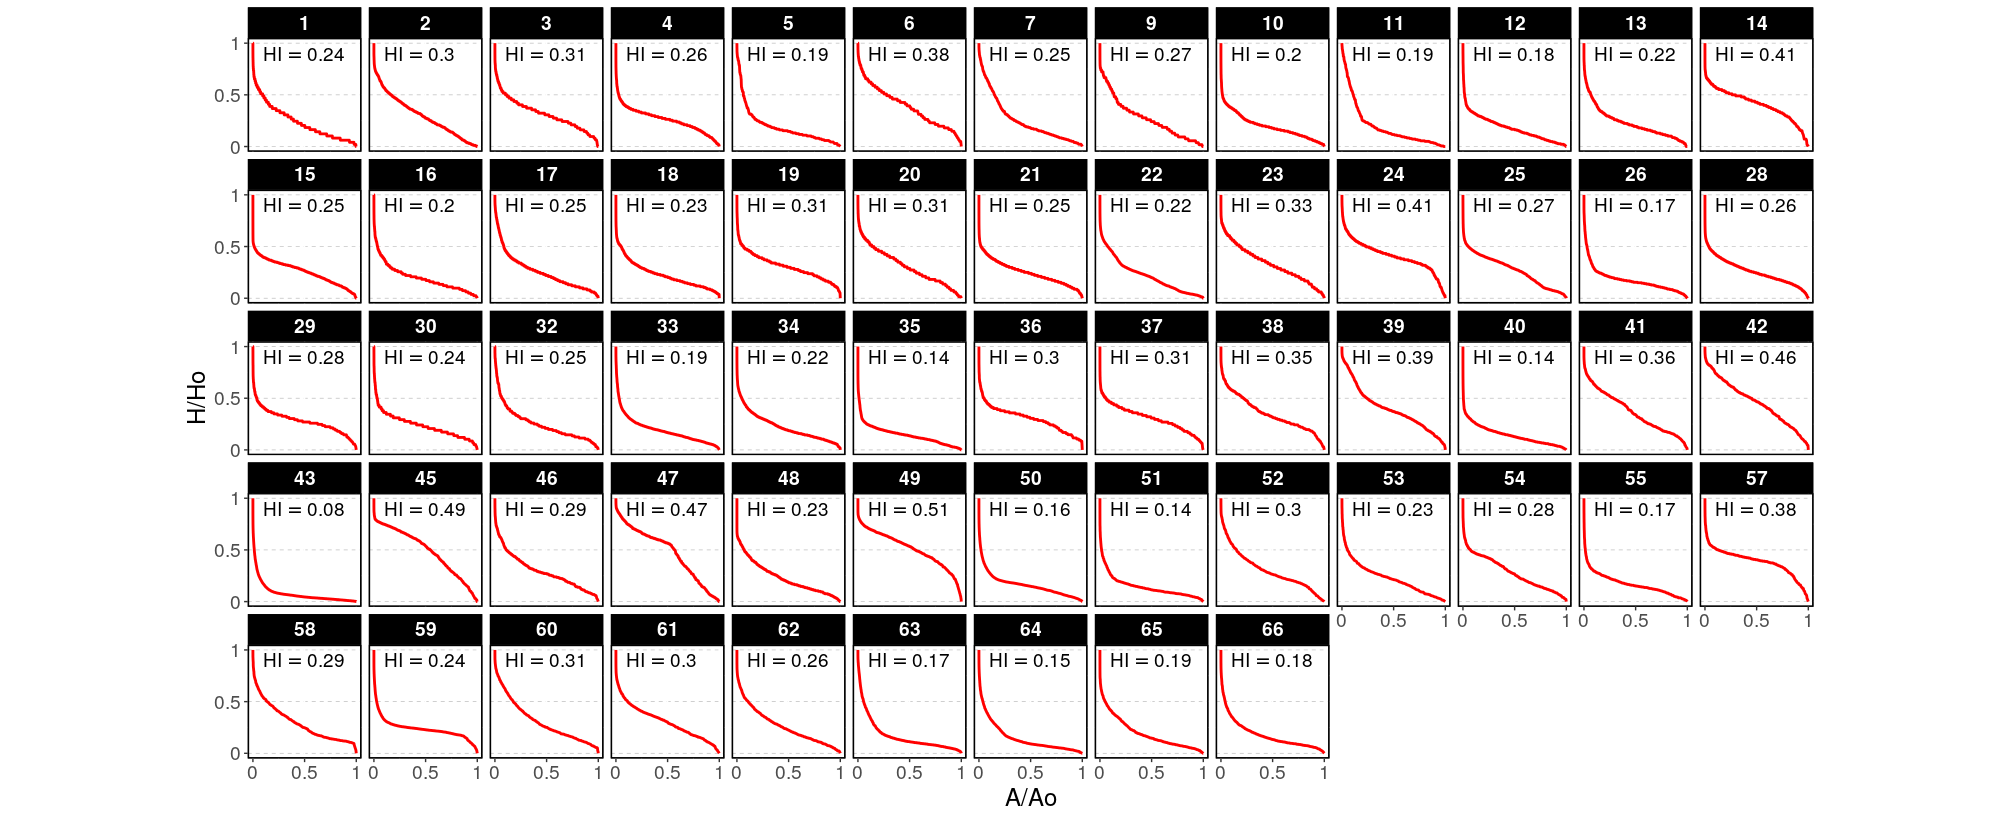
\includegraphics[width=1.10000\textwidth]{HypsoBasinOrder2.png}
\caption{Curva e integral hipsométrica para las cuencas de orden
2\label{hypsob2}}
\end{figure}

\begin{figure}
\centering
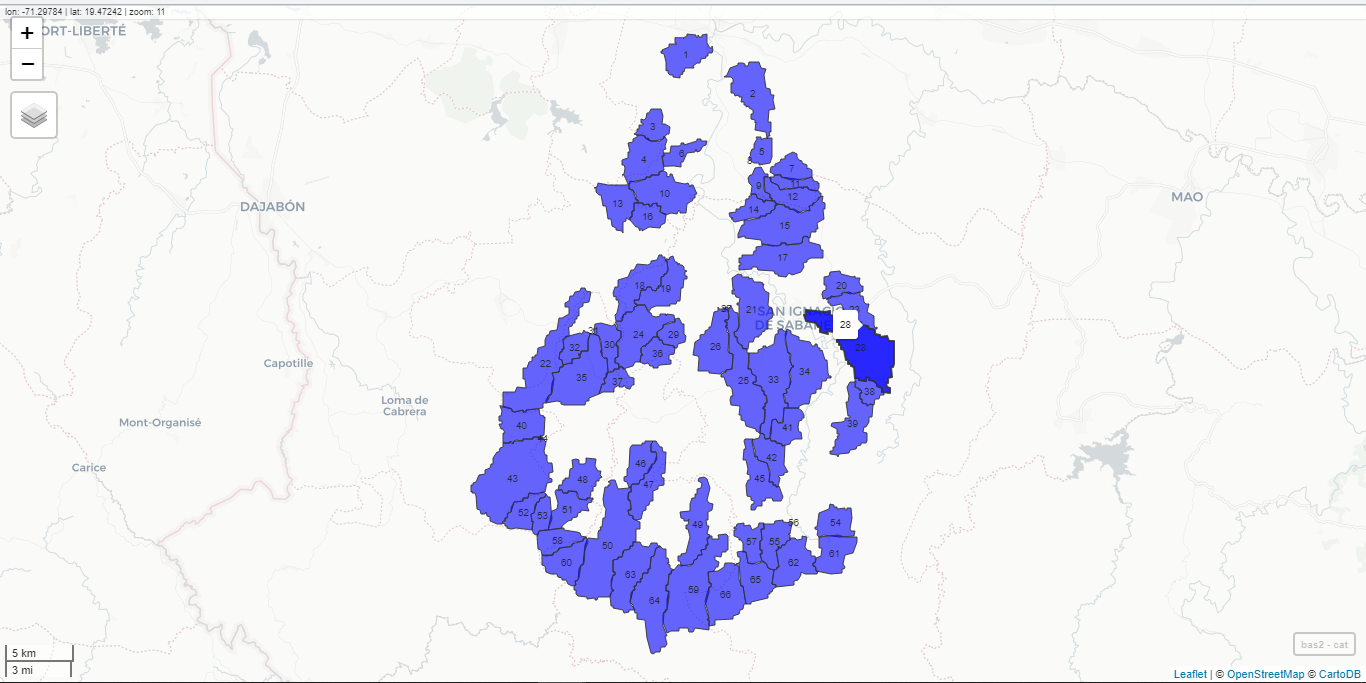
\includegraphics[width=0.90000\textwidth]{Mapview_hypsobasinorder2.png}
\caption{Cuencas de red de drenaje orden 2\label{hypb2}}
\end{figure}

\begin{figure}
\centering
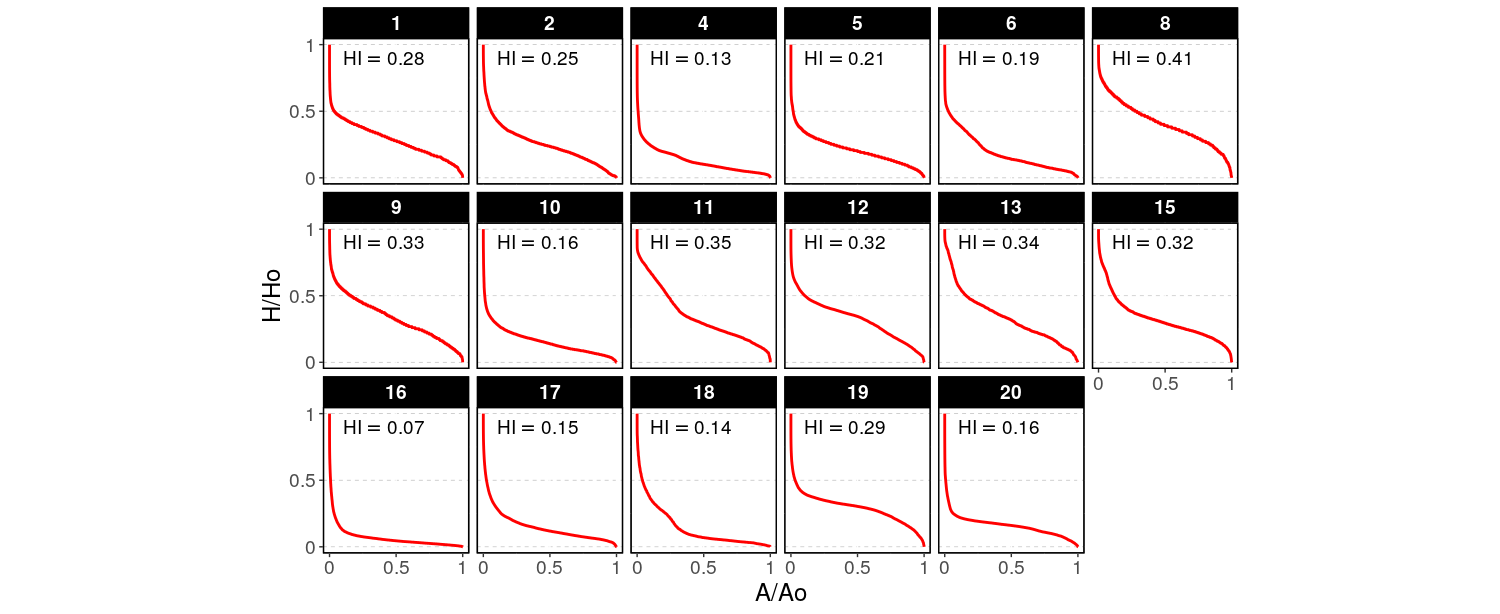
\includegraphics[width=1.00000\textwidth]{HypsoBasinOrder3.png}
\caption{Curva e integral hipsométrica para las cuencas de orden
3\label{hysob3}}
\end{figure}

\begin{figure}
\centering
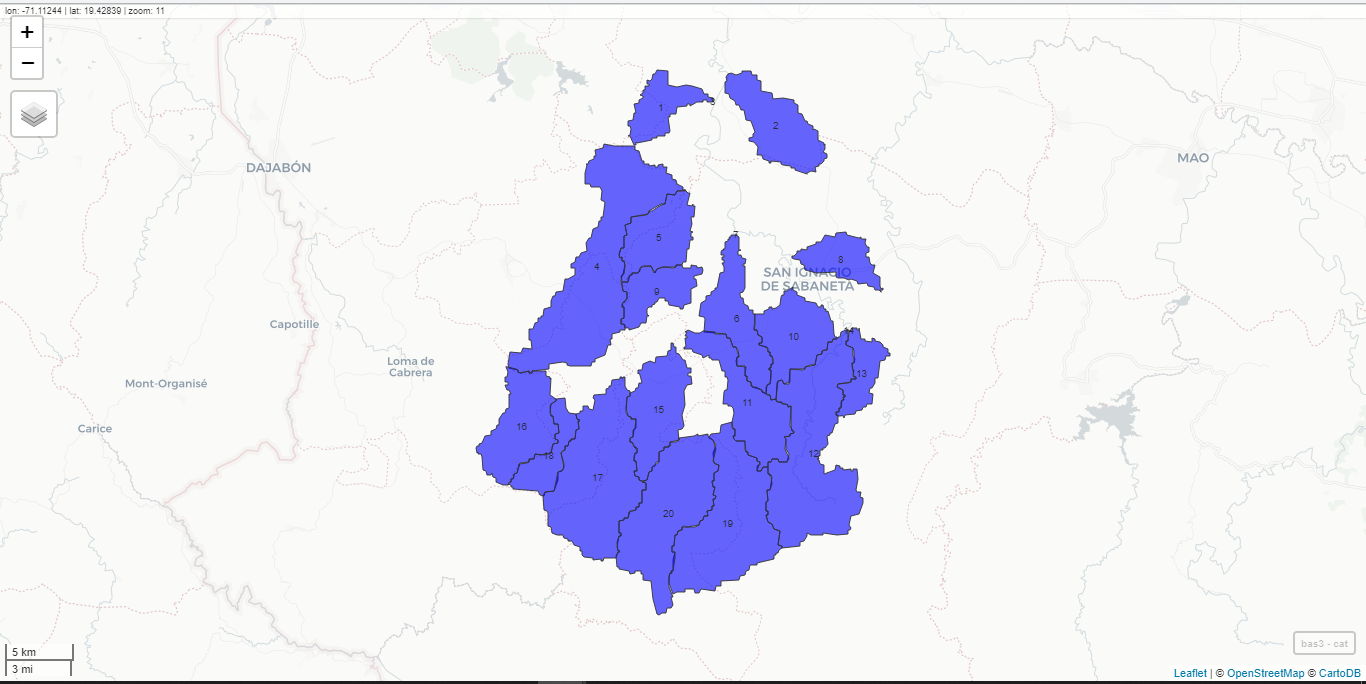
\includegraphics[width=0.90000\textwidth]{Mapview_hypsobasinorder3.png}
\caption{Cuencas de red de drenaje orden 3\label{hypb3}}
\end{figure}

\section{Discusión}\label{discusiuxf3n}

Con los hallazgos producidos sobre la cuenca del rio Guayubin, es
posible responder a las preguntas planteadas sobre la forma de la cuenca
y su red de drenaje, los patrones en la red de drenaje, la organizacion
de la red de drenaje, el fenomeno de constancia, la relacion de los
perfiles longitudinales y su indice de concavidad con la litologia en la
cuenca, la relacion de los parametros de cuenca con la litologia, al
igual que la relacion de la curva hipsometrica y la integral con la
litologia. Ademas, es posible hacer comparaciones de eficacia del metodo
empleado para extraer las redes de drenaje con el mapa topologico de
Republica Dominicana (s.a. (s.f.)).

En los parametros de cuenca y en las estadisticas de ordenes de red, el
valor de area de cuenca se mantuvo sin cambios; pero comparandolos con
las informaciones extraidas de Medio Ambiente y Recurso Naturales (2015)
los valores que se obtuvieron no concuerdan, puesto que, la cuenca
presentada por Medio Ambiente y Recurso Naturales (2015) es mas pequeña
que la producida por los algoritmos en R (ver tablas
\ref{tab:parametrosm} y \ref{tab:estadisticaor}.

La cuenca tiene forma de pera (Terrain Works (2014)) y la forma de su
red de drenaje es dendrítica (Gutiérrez Elorza (2008)). La forma de la
red de drenaje se produce en zonas de relieve heterogeneo como se
presenta la parte de cuenca alta; los cursos de agua se desarrollan
libremente y no depende de un control estructurales (Ingeniero Civil
(2018)); la cuenca esta asentuada en rocas de tipo igneas o magmaticas y
sedimentarias (Mollat (2004)). Howard (1967) asegura que lospatrones
denditricos los sedimentos tienen una resistencia uniforme.

La red de drenaje de la cuenca presenta signos de haber sufrido el
fenómeno de reorganización captura fluvial, según Pastor (2013) este
fenomeno se puede identificar al observar la red de drenaje, donde se
producen cambios abruptos en el recorrido del cauce que ha sido captura.
Se ha observado que este fenómeno se produce en todas las redes desde
orden 1 a orden 5, en especial en las redes de orden mas bajo, pero
puede verse muy marcado en la red de orden cinco, donde se produce
cambios del tipo de roca y relieve es ma heterogeneo (ver
figura\ref{grosor} y \ref{magecu}).

Según Summerfield (1991), la razon de bifurcacion que esta entre 3 y 5,
indica que la litologia del lugar es homogenea. En tabla \ref{razones},
es visible como los valores para la razon de bifurcacion en los ordenes
de red difieren el uno del otro, los ordenes 1, 2, 3 y 4 mantienen una
homogeneidad en su litogia. Como se observa en las tablas
\ref{tab:regresionc} y ref\{tab:estandard\}, las razones de bifurcacion
obtenidas se corresponden. Ambos valores coinciden con la razon de
bifurcacion calculada con codigo en R (4.064346), podemos concluir que
mantienen una constancia en el tipo de roca presente.

Los cursos mas largos de la red de drenaje que tienen los mas altos
indices de concavidad fueron los cursos 30, 48, 52, 55 y 56 (0.59; 0.51;
0.51; 0.54; y 0.47, respectivamente), lo que indica que hubo un cambio
en el trayecto que recorren esos cursos de agua que este relacionado a
la aparicion de una roca dura, tras haber comparado los resultados de
los cursos mas largo en el mapa geologico nacional (Mollat (2004)), se
comprueba que existe un cambio en la litologia presente en los cursos de
agua, en el caso del curso 30 con un indice de 0.59 de concavidad, al
pasar de estar sobre rocas tonalitas a estar sobre rocas sedimentarias y
de originadas en arcos de islas se produce un cambio en su trayectoria.
Tambien se vio afectado el curso de agua 19, quien presenta un indice
concavidad de 0.46 producto de que este flujo en su trayecto se
encuentra con una falla tectonica, provocando el cambio en su curso. Y
los cursos mas rectilineos con los indices de concavidad mas bajos son
los cursos de agua numero 15, 16, 23 y 38, con valores menores a 0.03,
estos cursos de agua realizan su reccorrido por un mismo tipo de roca
por lo que no experimenta cambios bruscos en su curso (ver
figura\ref{lfpnet}, \ref{plongitudinal} y \ref{indicec}).

Los parametros morfometricos obtenidos con \texttt{r.basin} (ver tabla
\ref{parametrosm}), indican que la elevacion minima en la cuenca del rio
Guayubin es 30.97 mslm y la maxima es 1396.73 mslm, por lo que existe
una diferencia de elevacion en la cuenca de 1365.76 m; mientras que su
elevacion media fue de 276.70. El parametro coeficiente de compacidad es
4.9 lo que indica que la forma de la superficie de la cuenca de acuerdo
a su delimitacion, y el predominio en su escorrentia, es muy alargada
(López Cadenas de Llano \& Mintegui Aguirre (1986)); pero, el parametro
forma de la cuenca genero un indice de 12.48 lo que indica que la cuenca
ademas de ser muy alargada, esta bastantante ensanchada en las zonas de
cuenca alta y cuenca media (Córdova (2016), y Pérez (1979)). Segun los
resultados de la razon de elongacion (0.50), se confirma que la cuenca
es alargada (De Matauco (2004)). El curso mas largo de la red de drenaje
o curso principal en la cuenca producido por \texttt{r.basin} tiene una
longitud 61.96 km; segun una comparacion realizada entre el el vectorial
de cursos mas largo (ver figura\ref{lfpnet}), y el curso que se obtuvo
con \texttt{r.basin} (ver figura\ref{vectoresrbasin}), es el curso
numero 30 obtenido con la funcion \texttt{LfpNetwork}. Por lo que la
cabecera del rio Guayubin se localiza al sureste de la indicada por
Medio Ambiente y Recurso Naturales (2015), bajo el nombre de Dajao.

La curva y la integral hipsométrica muestran la reparticion de
elevaciones en la cuenca (Jose Ramon Martinez Batlle (2019)). El valor
minimo generado para la integral hipsometrica fue 0.08 en el curso 43.
En tanto, el valor maximo para la integra fue de 0.48 en el curso 45
(ver tabla \ref{ihco2}). Y los curso mas curvos fueron 37 y 18. El
primero presenta signos de una evolucion lenta en su elevacion; y el
segundo, presenta una evolucion media en su elevacion. Ver
figuras\ref{hypsob2} y \ref{hypb2}. Los cursos 41 y 42 son los mas
rectilineo y su integral hipsometrica es moderada por lo que estos
cursos han experimentado poca evolucion rapida en su elevacion.

Los cursos de agua pertenecientes a la cuencas de orden 3, los valores
maximos presentes (8 y 13), tuvieron una evolucion media en la
elevacion. Y los cursos 4 y 16, demuestran una lenta y estable evolucion
en la elevacion (ver tabla \ref{ihco3}). Ver figuras \ref{hysob3} y
\ref{hypb3}.

Toda la informacion generada sobre la cuenca sirve como perdaño a
futuras investigaciones sobre la misma u otras cuencas fluviales en el
pais.

El estudio esta limitado a los analisis cuantitativos, puesto que carece
de la toma de muestras en campo para una mas precisa comprension de la
cuenca.

\section{Agradecimientos}\label{agradecimientos}

A Dios por la fuerza y la salud que me ha dado durante todo este tiempo,
sin dejarme caer.

A mi maestro \texttt{Jose\ Martinez\ Battle} por el apoyo incondicional,
tanto emocional como tecnico, por ser guia durante todo el trayecto, por
ser paciente, y sobre todo por su disponibilidad para colaborar.

A mi companero de carrera y amigo \texttt{Welifer\ Lebron} por su
asesoramiento.

A mis companeros
\texttt{Saderis\ Carmona,\ Franklin\ Gomez,\ Randy\ Mueses,\ Frank\ de\ la\ Cruz\ y\ Cinthia\ Vanderpool}
quienes estuvieron presente en este nuevo reto en el que nos embarcamos
tres meses atras, y de los cuales he recibido apoyo emocional y tecnico,
tambien por sus maneras de ayudarnos entre si a liberar estres.

A mi madre \texttt{Denny\ Laureano}, mis hermanos
\texttt{Darleny\ Linares,\ Dihana\ Carolina\ Linares\ y\ Jose\ Daniel\ Linares}
por la comprension y el apoyo tanto moral como emocional durante este
tiempo.

A mis amistades por el apoyo, comprension y motivacion para que continue
mis proyectos.

\section{Información de soporte}\label{informaciuxf3n-de-soporte}

\section{\texorpdfstring{\emph{Script}
reproducible}{Script reproducible}}\label{script-reproducible}

\section*{Referencia}\label{referencia}
\addcontentsline{toc}{section}{Referencia}

\hypertarget{refs}{}
\hypertarget{ref-Hypsocjose}{}
Batlle, J. R. M. (2018a). \emph{Función hypsointcurve}. Retrieved from
\url{https://github.com/geofis/rgrass/blob/master/integral_hypsometric_curve.R}

\hypertarget{ref-lfpnetjose}{}
Batlle, J. R. M. (2018b). \emph{Función lfpnetwork}. Retrieved from
\url{https://github.com/geofis/rgrass/blob/master/lfp_network.R}

\hypertarget{ref-lfpconcajose}{}
Batlle, J. R. M. (2018c). \emph{Función lfpprofilesconcavity}. Retrieved
from
\url{https://github.com/geofis/rgrass/blob/master/lfp_profiles_concavity.R}

\hypertarget{ref-xyvector}{}
Batlle, J. R. M. (2018d). \emph{Función xyvector}. Retrieved from
\url{https://raw.githubusercontent.com/geofis/rgrass/master/xyvector.R}

\hypertarget{ref-batlle2019drainage}{}
Batlle, J. R. M. (2019). \emph{Drainage rearrangement as a driver of
geomorphological evolution during the upper pleistocene in a small
tropical basin}.

\hypertarget{ref-intext}{}
Batlle, J. R. M. (2020a). \emph{Función integerextent}. Retrieved from
\url{https://raw.githubusercontent.com/geofis/rgrass/master/integerextent.R}

\hypertarget{ref-Mytransjose}{}
Batlle, J. R. M. (2020b). \emph{Función my-trans}. Retrieved from
\url{https://github.com/geomorfologia-master/unidad-4-asignacion-1-procesos-fluviales/blob/master/my-trans.R}

\hypertarget{ref-bowden1964effect}{}
Bowden, K. L., \& Wallis, J. R. (1964). Effect of stream-ordering
technique on horton's laws of drainage composition. \emph{Geological
Society of America Bulletin}, \emph{75}(8), 767--774.

\hypertarget{ref-castillo2015delimitacion}{}
Castillo, F. A. J. (2015). Delimitación automática de microcuencas
utilizando datos srtm de la nasa. \emph{Enfoque UTE}, \emph{6}(4),
81--97.

\hypertarget{ref-wateroutlet}{}
Charles Ehlschlaeger, U. A. C. E. R. L. (2003--2021a). \emph{Addon
r.water.outlet}. Retrieved from
\url{https://grass.osgeo.org/grass78/manuals/r.water.outlet.html}

\hypertarget{ref-watershedcharles}{}
Charles Ehlschlaeger, U. A. C. E. R. L. (2003--2021b). \emph{Addon
r.watershed}. Retrieved from
\url{https://grass.osgeo.org/grass79/manuals/r.watershed.html}

\hypertarget{ref-christofoletti1988geomorfologia}{}
Christofoletti, A. (1988). \emph{Geomorfologia}. Editora Blucher.

\hypertarget{ref-cordova2016parametros}{}
Córdova, M. (2016). \emph{Parámetros geomorfológicos de cuencas
hidrográficas}. Obtenido de Prontubeam: http://www. prontubeam.
com/articulos/articulos. php.

\hypertarget{ref-de2004analisis}{}
De Matauco, A. I. G. (2004). Análisis morfométrico de la cuenca y de la
red de drenaje del río zadorra y sus afluentes aplicado a la
peligrosidad de crecidas. \emph{Boletín de La Asociación de Geógrafos
Españoles}, (38), 311--330.

\hypertarget{ref-ESRI2012}{}
ESRI, E. S. R. I. (2012). ArcGIS resources: Definir cuencas
hidrográficas. Retrieved from
\url{https://help.arcgis.com/es/arcgisdesktop/10.0/help/index.html\#//009z00000068000000}

\hypertarget{ref-fernandez2016analise}{}
Fernandez, O. V. Q., \& Rocha, A. S. da. (2016). Análise preliminar da
aplicação da integral hipsométrica à caracterização das unidades de
paisagem na bacia do paraná iii, oeste do paraná. \emph{Anais VIII
SIMPGEO-as Fronteiras Da Ciência Geográfica: Avanços E Possibilidades.
Marechal Cândido Rondon, N. November}, 497--506.

\hypertarget{ref-gdalwarp}{}
Frank Warmerdam, Even Rouault, \& others. (1998--2021). \emph{Utility
gdalwarp}. Retrieved from \url{https://gdal.org/programs/gdalwarp.html}

\hypertarget{ref-garzonmorfologia}{}
Garzón Heydt, G., Ortega, J., Garrote, J., \& others. (n.d.).
\emph{Morfología de perfiles de ríos en roca. control tectónico y
significado evolutivo en el bajo guadiana}.

\hypertarget{ref-goldrick2007regional}{}
Goldrick, G., \& Bishop, P. (2007). Regional analysis of bedrock stream
long profiles: Evaluation of hack's sl form, and formulation and
assessment of an alternative (the ds form). \emph{Earth Surface
Processes and Landforms}, \emph{32}(5), 649--671.

\hypertarget{ref-gregory1973drainage}{}
Gregory, K. J., \& Walling, D. E. (1973). \emph{Drainage basin form and
process}.

\hypertarget{ref-gutierrez2008geomorfologia}{}
Gutiérrez Elorza, M. (2008). \emph{Geomorfología}.

\hypertarget{ref-horton1945erosional}{}
Horton, R. E. (1945). Erosional development of streams and their
drainage basins; hydrophysical approach to quantitative morphology.
\emph{Geological Society of America Bulletin}, \emph{56}(3), 275--370.

\hypertarget{ref-howard1967drainage}{}
Howard, A. D. (1967). Drainage analysis in geologic interpretation: A
summation. \emph{AAPG Bulletin}, \emph{51}(11), 2246--2259.

\hypertarget{ref-patron2018}{}
Ingeniero Civil, team. (2018). Patrones de drenaje y su significado.
Retrieved from
\url{https://www.cuevadelcivil.com/2011/06/diseno-de-drenaje-y-su-significacion.html}

\hypertarget{ref-streambasinsjareck}{}
Jarek Jasiewicz, G., Adam Mickiewicz University, \& Institute, G.
(2003--2021a). \emph{Addon r.stream.basins}. Retrieved from
\url{https://grass.osgeo.org/grass78/manuals/addons/r.stream.basins.html}

\hypertarget{ref-streamstats}{}
Jarek Jasiewicz, G., Adam Mickiewicz University, \& Institute, G.
(2003--2021b). \emph{Addon r.stream.stats}. Retrieved from
\url{https://grass.osgeo.org/grass78/manuals/addons/r.stream.stats.html}

\hypertarget{ref-streamorder}{}
Jasiewicz, J. (2003--2021). \emph{Addon r.stream.order}. Retrieved from
\url{https://grass.osgeo.org/grass78/manuals/addons/r.stream.order.html}

\hypertarget{ref-gproj}{}
Kelly, P. (2003--2021). \emph{Addon g.proj}. Retrieved from
\url{https://grass.osgeo.org/grass79/manuals/g.proj.html}

\hypertarget{ref-lopez1986hidrologia}{}
López Cadenas de Llano, F., \& Mintegui Aguirre, J. (1986).
\emph{Hidrología de la superficie-ti}.

\hypertarget{ref-EPSG}{}
MappingGis, D. A. (2016). Qué son los códigos epsg / srid y su
vinculación con postgis. Retrieved from
\url{https://mappinggis.com/2016/04/los-codigos-epsg-srid-vinculacion-postgis/}

\hypertarget{ref-basinmargherita}{}
Margherita Di Leo, M. D. S. (2003--2021). \emph{Addon r.basin}.
Retrieved from
\url{https://grass.osgeo.org/grass78/manuals/addons/r.basin.html\#morphometric-parameters-of-basin}

\hypertarget{ref-Mmar2015cuenca}{}
Medio Ambiente y Recurso Naturales, M. de. (2015). \emph{Cuenca río
yaque del norte y su zona costera}.
urlhttp://ambiente.gob.do/wp-content/uploads/2016/11/Yaque-del-Norte-Subcuencas-Hidrograficas-1.pdf.

\hypertarget{ref-streamnextractmarkus}{}
Metz, M. (2003--2021). \emph{Addon r.stream.extract}. Retrieved from
\url{https://grass.osgeo.org/grass78/manuals/r.stream.extract.html}

\hypertarget{ref-rinfo}{}
Michael O'Shea, U. A. C. E. R. L. (2003--2021). \emph{Addon r.info}.
Retrieved from \url{https://grass.osgeo.org/grass78/manuals/r.info.html}

\hypertarget{ref-Mollat2004mapa}{}
Mollat, W., H. (2004). \emph{Mapa geológico nacional de la república
dpminicana: Escala 1:250,000}.
urlhttps://geofis.xyz/lm/index.php/view/map/?repository=geo250krd\&project=geologico\_gpkg.

\hypertarget{ref-morais2010geomorfologia}{}
Morais, F., \& Almeida, L. M. (2010). Geomorfologia fluvial da bacia
hidrográfica do ribeirão jaú-palmas-to. \emph{Brazilian Geographical
Journal: Geosciences and Humanities Research Medium}, \emph{1}(2).

\hypertarget{ref-pastor2013capturas}{}
Pastor, A. (2013). Las capturas fluviales: Contextos, causas y
consecuencias. una explicación de los procesos de captura fluvial en
distintos contextos geológicos. \emph{Revista de Geografía Espacios},
\emph{3}(5), 27--41.

\hypertarget{ref-pedraza1996geomorfologia}{}
Pedraza Gilsanz, J. de. (1996). \emph{Geomorfología: Principios, métodos
y aplicaciones}.

\hypertarget{ref-perez1979fundamentos}{}
Pérez, J. (1979). Fundamentos del ciclo hidrológico. \emph{Universidad
Central de Venezuela. Facultad de Ingeniería. Departamento de
Meteorología E Hidrología. Caracas. Venezuela}, 01--38.

\hypertarget{ref-pinilla1993symposium}{}
Pinilla, A. (1993). \emph{Symposium sobre la raña en españa y portugal}
(Vol. 2). Editorial CSIC-CSIC Press.

\hypertarget{ref-TopoMap}{}
s.a. (s.f.). \emph{Topo map of the dominican republic 1:50k}.
urlhttps://geofis.xyz/lm/index.php/view/map/?repository=mtnrd50k\&project=mtnrd50k.

\hypertarget{ref-strahler1952hypsometric}{}
Strahler, A. N. (1952). Hypsometric (area-altitude) analysis of
erosional topography. \emph{Geological Society of America Bulletin},
\emph{63}(11), 1117--1142.

\hypertarget{ref-summerfield1991sub}{}
Summerfield, M. (1991). Sub-aerial denudation of passive margins:
Regional elevation versus local relief models. \emph{Earth and Planetary
Science Letters}, \emph{102}(3-4), 460--469.

\hypertarget{ref-tovect}{}
Team, G. D. (2003--2021). \emph{Addon r.to.vect}. Retrieved from
\url{https://grass.osgeo.org/grass76/manuals/r.to.vect.html}

\hypertarget{ref-tributary}{}
Terrain Works, T. (2014). Tributary confluence effects. Retrieved from
\url{http://www.netmaptools.org/Pages/NetMapHelp/tributary_confluence_effects.htm}

\hypertarget{ref-venkatachalam2001automatic}{}
Venkatachalam, P., Mohan, B., Kotwal, A., Mishra, V., Muthuramakrishnan,
V., \& Pandya, M. (2001). Automatic delineation of watersheds for
hydrological applications proc. \emph{ACRS 2001-22nd asian conference on
remote sensing, 5-9 november 2001, singapore. vol}, \emph{2},
1096--1101.

\hypertarget{ref-ringdal}{}
Warmerdam, F. (2003--2021). \emph{Addon r.in.gdal}. Retrieved from
\url{https://grass.osgeo.org/grass79/manuals/r.in.gdal.html}

\hypertarget{ref-wikipedia2020stream}{}
Wikipedia, C. (2020). Stream order. Retrieved from
\url{https://en.wikipedia.org/wiki/Stream_order}




\newpage
\singlespacing 
\end{document}
